\documentclass{article}
\usepackage[a2paper, landscape, margin = 0in]{geometry}
\usepackage{multicol}
\usepackage{amsmath}
\usepackage{amsfonts}
\usepackage{tikz}
\usetikzlibrary{decorations.pathmorphing}
\usepackage{amsmath,amssymb}

\usepackage{mathtools}
\usepackage{amsmath,amssymb}

\usepackage[utf8]{inputenc}
\tikzstyle{mybox} = [draw=black, fill=white, very thick,
    rectangle, rounded corners, inner sep=10pt, inner ysep=10pt]
\tikzstyle{fancytitle} =[fill=black, text=white, font=\bfseries]
\begin{document}

\begin{center}{\huge{\textbf{Computational biophysics}}}\\
\end{center}
\noindent
\begin{multicols*}{4}
\noindent
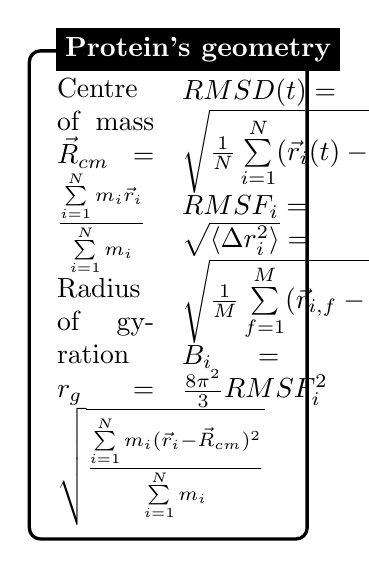
\begin{tikzpicture}
    \node [mybox] (box){%
        \begin{minipage}{0.233\textwidth}
            \begin{multicols}{2}
                Centre of mass $\vec{R}_{cm} = \frac{\sum\limits_{i=1}^Nm_i\vec{r}_i}{\sum\limits_{i=1}^Nm_i}$ \\
                Radius of gyration $r_g = \sqrt{\frac{\sum\limits_{i=1}^Nm_i(\vec{r}_i-\vec{R}_{cm})^2}{\sum\limits_{i=1}^Nm_i}}$\\
                $RMSD(t) = \sqrt{\frac{1}{N}\sum\limits_{i=1}^N(\vec{r}_{i}(t)-\vec{r}_{i}(0))^2}$\\
                $RMSF_i = \sqrt{\langle\Delta r_i^2\rangle} = \sqrt{\frac{1}{M}\sum\limits_{f=1}^M(\vec{r}_{i,f}-\langle\vec{r}_i\rangle)^2}$\\
                $B_i = \frac{8\pi^2}{3}RMSF_i^2$\\
            \end{multicols}
        \end{minipage}
    };
    \node[fancytitle, right=10pt] at (box.north west) {Protein's geometry};
\end{tikzpicture}
\begin{tikzpicture}
    \node [mybox] (box){%
        \begin{minipage}{0.233\textwidth}

            \begin{tikzpicture}
                \node [mybox] (box1){%
                    \begin{minipage}{0.95\textwidth}
                        Harmonic $U(r_{AB}) = \frac{1}{2}k_{AB}(r_{AB}-r_{AB,eq})^2$\\
                        Anarmonic $U(r_{AB}) = \frac{1}{2}\left[k_{AB} + k_{AB}^{(3)}(r_{AB}-r_{AB,eq})\right](r_{AB}-r_{AB, eq})^2$\\
                        Quartic correction $\begin{aligned}U(r_{AB}) = \frac{1}{2}&\left[k_{AB} + k_{AB}^{(3)}(r_{AB}-r_{AB,eq}) + k_{AB}^{(4)}(r_{AB}-r_{AB,eq})^2\right]\cdot\\
                            &\cdot(r_{AB}-r_{AB, eq})^2\end{aligned}$\\
                        Morse $U(r_{AB}) = D_{AB}\left[1-e^{-\alpha_{AB}(r_{AB}-r_{AB,eq}^2)}\right]$\\
                    \end{minipage}
                };
                \node[fancytitle, inner sep = 1pt, right=10pt] at (box1.north west) { Bond stretching};
            \end{tikzpicture}
            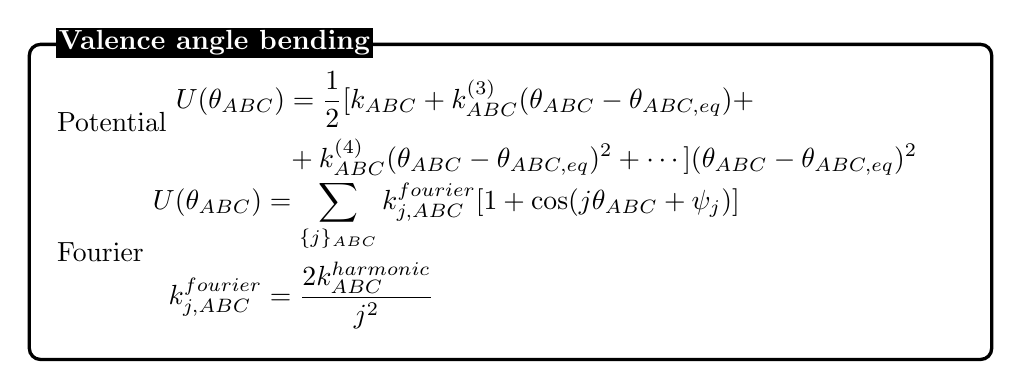
\begin{tikzpicture}
                \node [mybox] (box1){%
                    \begin{minipage}{0.95\textwidth}
                        Potential $\begin{aligned}U(\theta_{ABC}) &= \frac{1}{2}[k_{ABC}+k^{(3)}_{ABC}(\theta_{ABC}-\theta_{ABC,eq})+\\
                        &+k^{(4)}_{ABC}(\theta_{ABC}-\theta_{ABC,eq})^2+\cdots](\theta_{ABC}-\theta_{ABC, eq})^2\end{aligned}$\\
                            Fourier $\begin{aligned}U(\theta_{ABC}) &= \sum\limits_{\{j\}_{ABC}}k^{fourier}_{j,ABC}[1+\cos(j\theta_{ABC}+\psi_j)]\\
                                k_{j, ABC}^{fourier} &= \frac{2k^{harmonic}_{ABC}}{j^2}\end{aligned}$\\

                    \end{minipage}
                };
                \node[fancytitle, inner sep = 1pt, right=10pt] at (box1.north west) {Valence angle bending};
            \end{tikzpicture}
            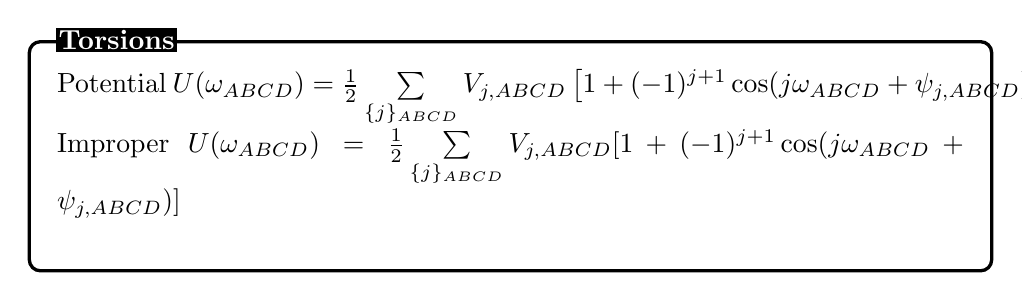
\begin{tikzpicture}
                \node [mybox] (box1){%
                    \begin{minipage}{0.95\textwidth}
	                Potential $U(\omega_{ABCD}) = \frac{1}{2}\sum\limits_{\{j\}_{ABCD}}V_{j,ABCD}\left[1+(-1)^{j+1}\cos(j\omega_{ABCD}+\psi_{j,ABCD})\right]$\\
                        Improper $U(\omega_{ABCD}) = \frac{1}{2}\sum\limits_{\{j\}_{ABCD}}V_{j,ABCD}[1+(-1)^{j+1}\cos(j\omega_{ABCD}+\psi_{j,ABCD})]$\\
                    \end{minipage}
                };
                \node[fancytitle, inner sep = 1pt, right=10pt] at (box1.north west) {Torsions};
            \end{tikzpicture}
            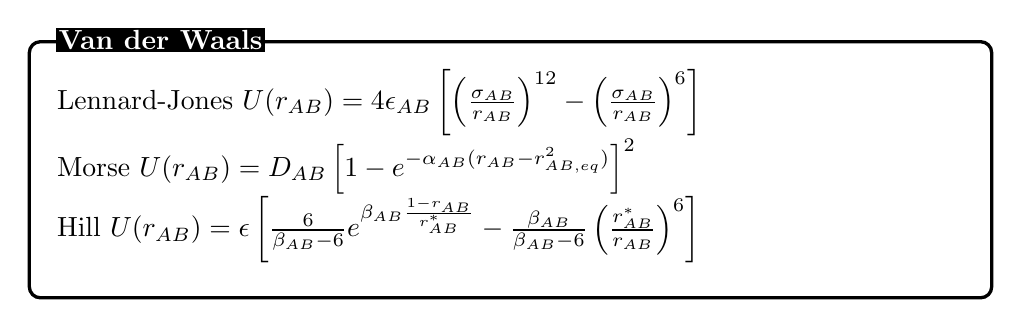
\begin{tikzpicture}
                \node [mybox] (box1){%
                    \begin{minipage}{0.95\textwidth}
                        Lennard-Jones $U(r_{AB}) = 4\epsilon_{AB}\left[\left(\frac{\sigma_{AB}}{r_{AB}}\right)^{12}-\left(\frac{\sigma_{AB}}{r_{AB}}\right)^6\right]$\\
                        Morse $U(r_{AB}) = D_{AB}\left[1-e^{-\alpha_{AB}(r_{AB}-r_{AB,eq}^2)}\right]^2$\\
                        Hill $U(r_{AB}) = \epsilon\left[\frac{6}{\beta_{AB}-6}e^{\beta_{AB}\frac{1-r_{AB}}{r^*_{AB}}}-\frac{\beta_{AB}}{\beta_{AB}-6}\left(\frac{r^*_{AB}}{r_{AB}}\right)^6\right]$\\
                    \end{minipage}
                };
                \node[fancytitle, inner sep = 1pt, right=10pt] at (box1.north west) {Van der Waals};
            \end{tikzpicture}
            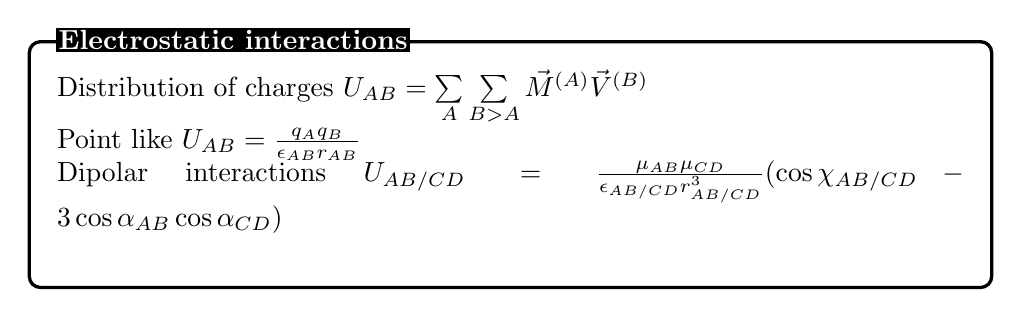
\begin{tikzpicture}
                \node [mybox] (box1){%
                    \begin{minipage}{0.95\textwidth}
                        Distribution of charges $U_{AB} = \sum\limits_A\sum\limits_{B>A}\vec{M}^{(A)}\vec{V}^{(B)}$\\
                        Point like $U_{AB} = \frac{q_Aq_B}{\epsilon_{AB}r_{AB}}$\\
                        Dipolar interactions $U_{AB/CD} = \frac{\mu_{AB}\mu_{CD}}{\epsilon_{AB/CD}r^3_{AB/CD}}(\cos\chi_{AB/CD}-3\cos\alpha_{AB}\cos\alpha_{CD})$\\
                    \end{minipage}
                };
                \node[fancytitle, inner sep = 1pt, right=10pt] at (box1.north west) {Electrostatic interactions};
            \end{tikzpicture}
            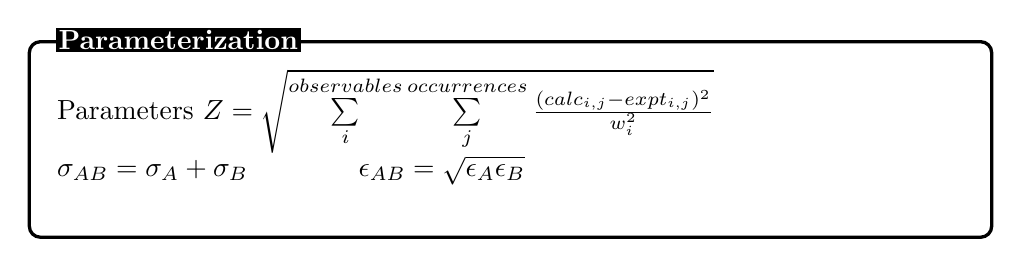
\begin{tikzpicture}
                \node [mybox] (box1){%
                    \begin{minipage}{0.95\textwidth}
                        Parameters $Z = \sqrt{\sum\limits_i^{observables}\sum\limits_j^{occurrences}\frac{(calc_{i,j}-expt_{i,j})^2}{w_i^2}}$\\
                        $\sigma_{AB} = \sigma_A + \sigma_B\qquad\qquad \epsilon_{AB} = \sqrt{\epsilon_A\epsilon_B}$\\
                    \end{minipage}
                };
                \node[fancytitle, inner sep = 1pt, right=10pt] at (box1.north west) {Parameterization};
            \end{tikzpicture}
        \end{minipage}
    };
    \node[fancytitle, right=10pt] at (box.north west) {Semi-empirical force fields};
\end{tikzpicture}
\begin{tikzpicture}
    \node [mybox] (box){%
        \begin{minipage}{0.233\textwidth}
            \begin{tikzpicture}
                \node [mybox] (box1){%
                    \begin{minipage}{0.95\textwidth}
                        $\vec{F} = m\vec{a}\qquad \vec{F}_{BA} = -\vec{F}_{AB}$\\
                        $\vec{v}(t) = \frac{d\vec{r}}{dt}\qquad \vec{a}(t) = \frac{d\vec{v}}{dt} = \frac{d^2\vec{r}}{dt^2}\qquad m\frac{d^2\vec{r}}{dt^2} = \vec{F}$\\
                        Force acting on atom $\vec{F}_i(\vec{r}_1, \dots, \vec{r}_N, \dot{\vec{r}}_i) = \sum\limits_{j\neq i}\vec{F}_{ij}(\vec{r}_i-\vec{r}_j)+\vec{F}^{(ext)}(\vec{r}_i, \dot{\vec{r}}_i)$\\
                        Bond stretching: $U = \frac{k_l}{2}(l-l^0)^2$\\
                        Bond bending: $U = \frac{k_\theta}{2}(\theta-\theta^0)^2$\\
                        Bond torsion: $U = k_\phi[1+\cos(n\phi-\phi^0)]$\\
                        Van der Waals interactions: $U = \biggl[\frac{a_{ij}}{r_{ij}^{12}}-\frac{b_{ij}}{r_{ij}^6}\biggr]$\\
                        Electrostatic interactions: $U = \frac{332q_iq_j}{\epsilon r_{ij}}$\\
                        $\vec{p}_i = m_i\vec{v}_i = m\dot{\vec{r}}_i\qquad \vec{F}_i = m_i\ddot{\vec{r}}_i = \dot{\vec{p}}_i$\\
                        $\vec{x}(t) = \{\vec{r}_1(t),\dots, \vec{r}_N(t), \vec{p}_1(t), \dots, \vec{p}_N(t)\}$\\
                    \end{minipage}
                };
                \node[fancytitle, inner sep = 1pt, right=10pt] at (box1.north west) {Newton's laws};
            \end{tikzpicture}
            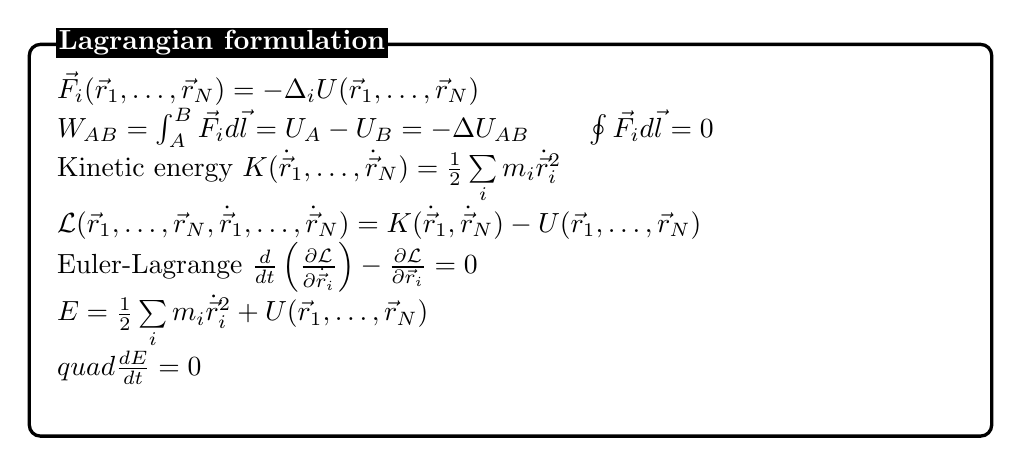
\begin{tikzpicture}
                \node [mybox] (box1){%
                    \begin{minipage}{0.95\textwidth}
                        $\vec{F}_i(\vec{r}_1, \dots, \vec{r}_N) = -\Delta_i U(\vec{r}_1, \dots, \vec{r}_N)$\\
                        $W_{AB} = \int_A^B\vec{F}_id\vec{l} = U_A - U_B = - \Delta U_{AB}\qquad \oint\vec{F}_id\vec{l}=0$\\
                        Kinetic energy $K(\dot{\vec{r}}_1, \dots, \dot{\vec{r}}_N) = \frac{1}{2}\sum\limits_{i}m_i\dot{\vec{r}}_i^2$\\
                        $\mathcal{L}(\vec{r}_1, \dots, \vec{r}_N, \dot{\vec{r}}_1, \dots, \dot{\vec{r}}_N) = K(\dot{\vec{r}}_1, \dot{\vec{r}}_N) - U(\vec{r}_1, \dots, \vec{r}_N)$\\
                        Euler-Lagrange $\frac{d}{dt}\left(\frac{\partial \mathcal{L}}{\partial\dot{\vec{r}}_i}\right) -\frac{\partial\mathcal{L}}{\partial\vec{r}_i} = 0$\\
                        $E = \frac{1}{2}\sum\limits_i m_i\dot{\vec{r}}_i^2 + U(\vec{r}_1, \dots, \vec{r}_N)\\quad \frac{dE}{dt} = 0$\\

                    \end{minipage}
                };
                \node[fancytitle, inner sep = 1pt, right=10pt] at (box1.north west) {Lagrangian formulation};
            \end{tikzpicture}
            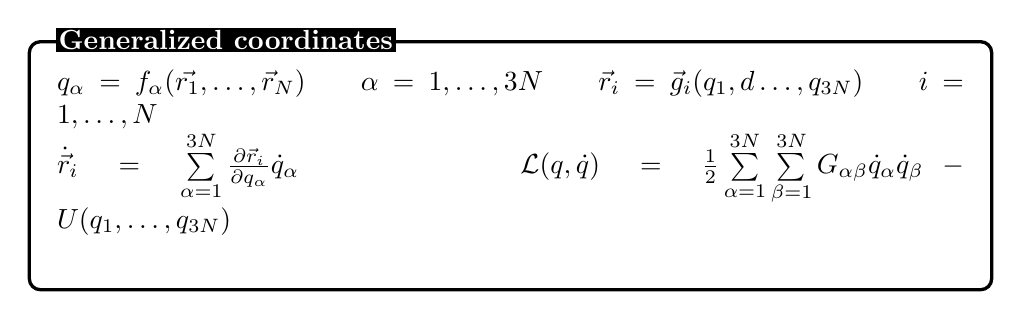
\begin{tikzpicture}
                \node [mybox] (box1){%
                    \begin{minipage}{0.95\textwidth}
	                $q_\alpha = f_\alpha(\vec{r_1}, \dots, \vec{r}_N)\qquad \alpha = 1, \dots, 3N\qquad\vec{r}_i =\vec{g}_i(q_1, d\dots, q_{3N})\qquad i =1, \dots, N$\\
                        $\dot{\vec{r}}_i = \sum\limits_{\alpha=1}^{3N}\frac{\partial \vec{r}_i}{\partial q_\alpha}\dot{q}_\alpha\qquad\qquad\qquad\qquad\mathcal{L}(q, \dot{q}) =\frac{1}{2}\sum\limits_{\alpha=1}^{3N}\sum\limits_{\beta=1}^{3N}G_{\alpha\beta}\dot{q}_\alpha\dot{q}_\beta - U(q_1, \dots, q_{3N})$\\
                    \end{minipage}

                };
                \node[fancytitle, inner sep = 1pt, right=10pt] at (box1.north west) {Generalized coordinates};
            \end{tikzpicture}


        \end{minipage}
    };
    \node[fancytitle, right=10pt] at (box.north west) {Classical mechanics};
\end{tikzpicture}
\begin{tikzpicture}
    \node [mybox] (box){%
        \begin{minipage}{0.233\textwidth}
            \begin{tikzpicture}
                \node [mybox] (box1){%
                    \begin{minipage}{0.95\textwidth}
                        $s = f'(x) \equiv g(x)\qquad f'(x) = g(x) = s\Rightarrow x = g^{-1}(s)$\\
                        $b(g^{-1}(s)) = f(g^{-1}(s))-sg^{-1}(s)\equiv\tilde{f}(s) = f(x(s))-sx(s)$\\
                        $\tilde{f}(s_1,\dots,s_n) = f(x_1(s_1, \dots, s_n),\dots x_n(s_1, \dots, s_n))-\sum\limits_i s_ix_i(s_1, \dots, s_n)$\;
                    \end{minipage}

                };
                \node[fancytitle, inner sep = 1pt, right=10pt] at (box1.north west) {Legendre transforms};
            \end{tikzpicture}
            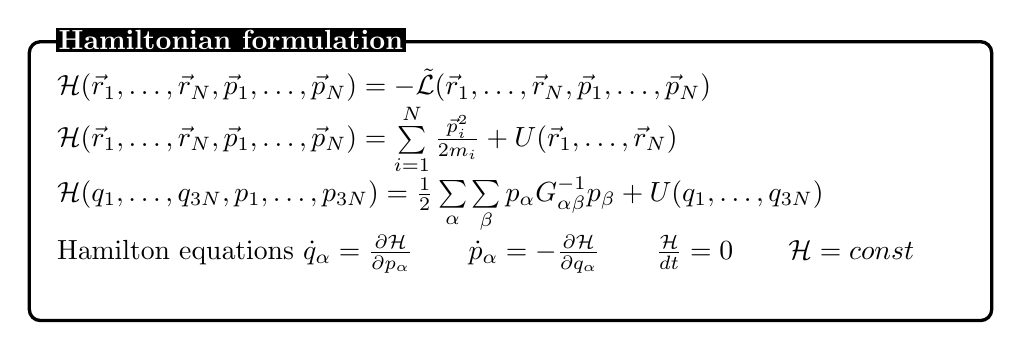
\begin{tikzpicture}
                \node [mybox] (box1){%
                    \begin{minipage}{0.95\textwidth}
                        $\mathcal{H}(\vec{r}_1, \dots, \vec{r}_N, \vec{p}_1, \dots, \vec{p}_N) = -\tilde{\mathcal{L}}(\vec{r}_1, \dots, \vec{r}_N, \vec{p}_1, \dots, \vec{p}_N)$\\
                        $\mathcal{H}(\vec{r}_1, \dots, \vec{r}_N, \vec{p}_1, \dots, \vec{p}_N) = \sum\limits_{i=1}^N\frac{\vec{p}_i^2}{2m_i} + U(\vec{r}_1, \dots, \vec{r}_N)$\\
                        $\mathcal{H}(q_1, \dots, q_{3N}, p_1, \dots, p_{3N}) =\frac{1}{2}\sum\limits_\alpha\sum\limits_\beta p_\alpha G_{\alpha\beta}^{-1}p_\beta + U(q_1, \dots, q_{3N})$\\
                        Hamilton equations $\dot{q}_\alpha = \frac{\partial\mathcal{H}}{\partial p_\alpha}\qquad\dot{p}_\alpha = -\frac{\partial\mathcal{H}}{\partial q_\alpha}\qquad\frac{\mathcal{H}}{dt} = 0\qquad\mathcal{H} = const$\\
                    \end{minipage}

                };
                \node[fancytitle, inner sep = 1pt, right=10pt] at (box1.north west) {Hamiltonian formulation};
            \end{tikzpicture}
            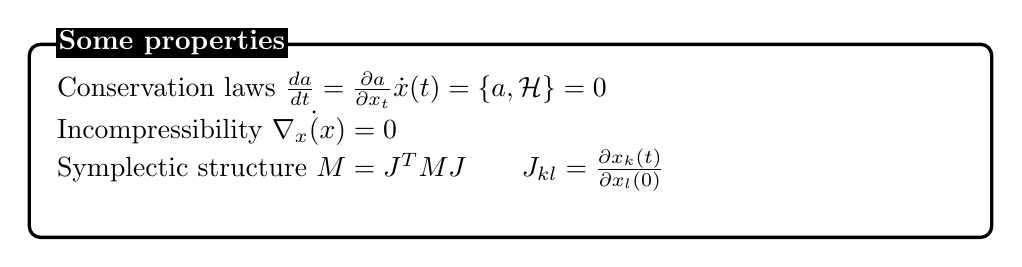
\begin{tikzpicture}
                \node [mybox] (box1){%
                    \begin{minipage}{0.95\textwidth}
                        Conservation laws $\frac{da}{dt} = \frac{\partial a}{\partial x_t}\dot{x}(t) = \{a, \mathcal{H}\} = 0$\\
                        Incompressibility $\nabla_x\dot(x) = 0$\\
                        Symplectic structure $M = J^TMJ\qquad J_{kl} = \frac{\partial x_k(t)}{\partial x_l(0)}$\\
                    \end{minipage}

                };
                \node[fancytitle, inner sep = 1pt, right=10pt] at (box1.north west) {Some properties};
            \end{tikzpicture}


        \end{minipage}
    };
    \node[fancytitle, right=10pt] at (box.north west) {Classical mechanics (contd)};
\end{tikzpicture}
\begin{tikzpicture}
    \node [mybox] (box){%
        \begin{minipage}{0.233\textwidth}
            \begin{tikzpicture}
                \node [mybox] (box1){%
                    \begin{minipage}{0.95\textwidth}
                        \begin{multicols}{2}
                            Equilibrium $g(N, P, V, T) = 0$\\
                            State function $f(n, P, V, T)$\\
                            Reversible work $dW_{rev} = -PdV+\mu dN$\\
                            Heat $dQ_{rev} = CdT$\\
                            First law $\Delta E = \Delta Q + \Delta W$\\
                            Entropy $\Delta S = \int_1^2\frac{dQ_{rev}}{T}$\\
                        \end{multicols}
                    \end{minipage}

                };
                \node[fancytitle, inner sep = 1pt, right=10pt] at (box1.north west) {Thermodynamics};
            \end{tikzpicture}
            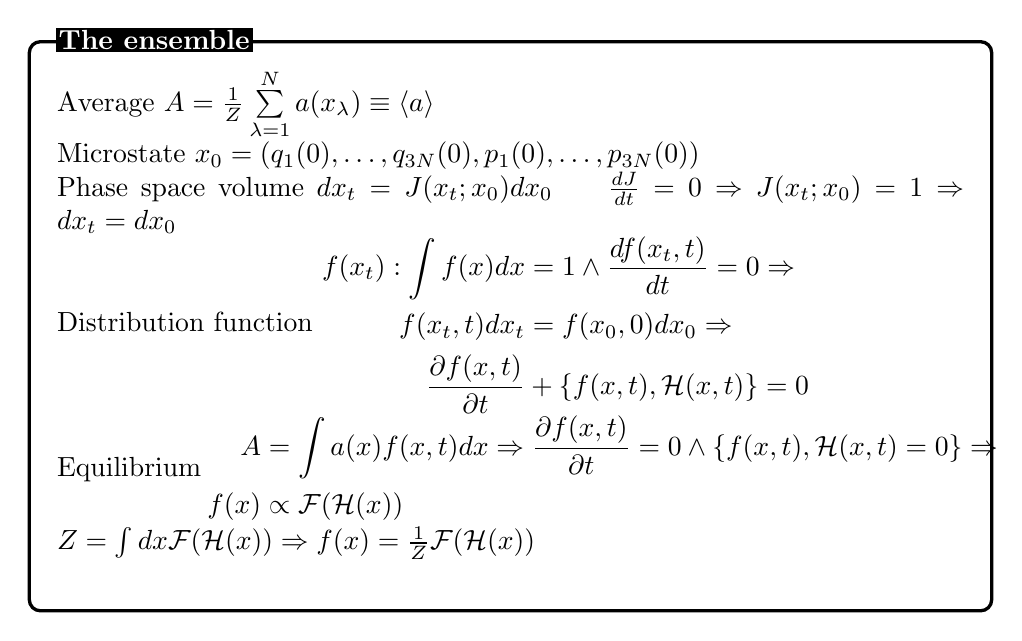
\begin{tikzpicture}
                \node [mybox] (box1){%
                    \begin{minipage}{0.95\textwidth}
                        Average $A = \frac{1}{Z}\sum\limits_{\lambda=1}^Na(x_\lambda)\equiv\langle a\rangle$\\
                        Microstate $x_0 = (q_1(0), \dots, q_{3N}(0), p_1(0), \dots, p_{3N}(0))$\\
                        Phase space volume $dx_t = J(x_t;x_0)dx_0\qquad \frac{dJ}{dt} = 0\Rightarrow J(x_t;x_0) = 1\Rightarrow dx_t=dx_0$\\
                        Distribution function $\begin{aligned}f(x_t):\int f(x)dx &= 1\land \frac{df(x_t,t)}{dt} = 0\Rightarrow\\ f(x_t, t)dx_t &= f(x_0,0)dx_0\Rightarrow\\\frac{\partial f(x,t)}{\partial t} &+ \{f(x,t), \mathcal{H}(x,t)\} = 0\end{aligned}$\\
                        Equilibrium $\begin{aligned}A &= \int a(x)f(x,t)dx\Rightarrow \frac{\partial f(x,t)}{\partial t} = 0\land \{f(x,t), \mathcal{H}(x,t) = 0\}\Rightarrow\\ f(x)&\propto\mathcal{F}(\mathcal{H}(x))\end{aligned}$\\
                        $Z = \int dx\mathcal{F}(\mathcal{H}(x))\Rightarrow f(x) = \frac{1}{Z}\mathcal{F}(\mathcal{H}(x))$\\
                    \end{minipage}

                };
                \node[fancytitle, inner sep = 1pt, right=10pt] at (box1.north west) {The ensemble};
            \end{tikzpicture}


        \end{minipage}

    };
    \node[fancytitle, right=10pt] at (box.north west) {Theoretical foundations of statistical mechanics};
\end{tikzpicture}
\begin{tikzpicture}
    \node [mybox] (box){%
        \begin{minipage}{0.233\textwidth}
            \begin{tikzpicture}
                \node [mybox] (box1){%
                    \begin{minipage}{0.95\textwidth}
                        State function $dS = \frac{1}{T}dE + \frac{P}{T}dV - \frac{\mu}{T}dN$\\
                        $\left(\frac{\partial S}{\partial E}\right)_{V, N} = \frac{1}{T}\qquad\left(\frac{\partial S}{\partial V}\right)_{N, E} = \frac{P}{T}\qquad\left(\frac{\partial S}{\partial N}\right)_{V, N} = \frac{\mu}{T}$\\
                        Boltzmann relation $S(N, V, E) = k\ln\omega(N, V, E)$\\
                        Distribution function $\begin{aligned}\Omega(N, V, E) &= M_N\int d\vec{p}\int_{D(V)}d\vec{r}\delta(\mathcal{H}(\vec{r}, \vec{p})-E) \\&= M_N\int dx\delta(\mathcal{H}(x)-E)\\ M_N &= \frac{E_0}{N!h^{3N}}\end{aligned}$\\
                        $A = \langle a\rangle = \frac{M_N}{\Omega(N, V, E)}\int dxa(x)\delta(\mathcal{H}(x)-E) = \frac{\int dxa()\delta(\mathcal{H}(x)-E)}{\int dx\delta(\mathcal{H}-E)}$\\
                        $\left\langle x_i\frac{\partial\mathcal{H}}{\partial x_j}\right\rangle = \frac{M_N}{\Omega(N, V, E)}\frac{\partial}{\partial E}\int_{\mathcal{H}(x)<E}dxx_i\frac{\partial(\mathcal{H}-E)}{\partial x_j}$\\
                    \end{minipage}

                };
                \node[fancytitle, inner sep = 1pt, right=10pt] at (box1.north west) {State and distribution function};
            \end{tikzpicture}
            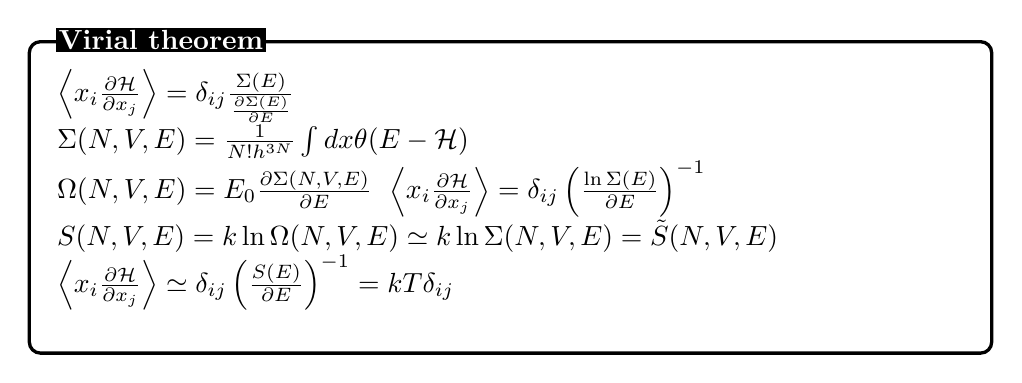
\begin{tikzpicture}
                \node [mybox] (box1){%
                    \begin{minipage}{0.95\textwidth}
                        $\left\langle x_i\frac{\partial\mathcal{H}}{\partial x_j} \right\rangle= \delta_{ij}\frac{\Sigma(E)}{\frac{\partial\Sigma(E)}{\partial E}}$\\
                        $\Sigma(N, V, E) = \frac{1}{N!h^{3N}}\int dx\theta(E-\mathcal{H})$\\
                        $\Omega(N, V, E) = E_0\frac{\partial\Sigma(N, V, E)}{\partial E}$\;
                        $\left\langle x_i\frac{\partial\mathcal{H}}{\partial x_j} \right\rangle= \delta_{ij}\left(\frac{\ln\Sigma(E)}{\partial E}\right)^{-1}$\\
                        $S(N,V,E) = k\ln\Omega(N, V, E)\simeq k\ln\Sigma(N, V, E)=\tilde{S}(N, V, E)$\\
                        $\left\langle x_i\frac{\partial\mathcal{H}}{\partial x_j} \right\rangle\simeq \delta_{ij}\left(\frac{S(E)}{\partial E}\right)^{-1} = kT\delta_{ij}$\\
                    \end{minipage}
                };
                \node[fancytitle, inner sep = 1pt, right=10pt] at (box1.north west) {Virial theorem};
            \end{tikzpicture}
            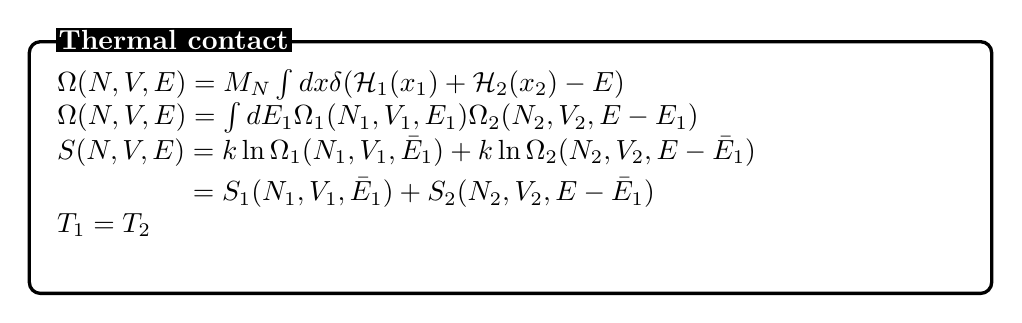
\begin{tikzpicture}
                \node [mybox] (box1){%
                    \begin{minipage}{0.95\textwidth}
                        $\Omega(N, V, E) = M_N\int dx\delta(\mathcal{H}_1(x_1) + \mathcal{H}_2(x_2)-E)$\\
                        $\Omega(N, V, E) = \int dE_1\Omega_1(N_1, V_1, E_1)\Omega_2(N_2, V_2, E-E_1)$\\
                        $\begin{aligned}S(N, V, E) &= k\ln\Omega_1(N_1,V_1, \bar{E}_1) + k\ln\Omega_2(N_2, V_2, E-\bar{E}_1) \\&=S_1(N_1, V_1, \bar{E}_1) + S_2(N_2,V_2,E-\bar{E}_1)\end{aligned}$\\
                        $T_1 = T_2$\\
                    \end{minipage}
                };
                \node[fancytitle, inner sep = 1pt, right=10pt] at (box1.north west) {Thermal contact};
            \end{tikzpicture}

        \end{minipage}

    };
    \node[fancytitle, right=10pt] at (box.north west) {Microcanonical ensemble};
\end{tikzpicture}
\begin{tikzpicture}
    \node [mybox] (box){%
        \begin{minipage}{0.233\textwidth}
            \begin{tikzpicture}
                \node [mybox] (box1){%
                    \begin{minipage}{0.95\textwidth}
                        $\vec{r}_i(t+\Delta t) = 2\vec{r}_i(t) - \vec{r}_i(t-\Delta t) + \frac{\Delta t^2}{m_i}\vec{F}_i(t)$\\
                        $\vec{v}_i(t+\Delta t) = \vec{v}_i(t) + \frac{\Delta t}{2m_i}\left[\vec{F}_i(t) + \vec{F}_i(t+\Delta t)\right]$\\
                        Initial conditions $f(v) = \sqrt{\frac{m}{2\pi kT}}e^{-\frac{mv^2}{2kT}}\qquad f(x) = \frac{1}{\sqrt{2\pi\sigma^2}}e^{-\frac{x^2}{2\sigma^2}}$\\
                    \end{minipage}
                };
                \node[fancytitle, inner sep = 1pt, right=10pt] at (box1.north west) {Verlet algorithm};
            \end{tikzpicture}
        \end{minipage}

    };
    \node[fancytitle, right=10pt] at (box.north west) {Introduction to molecular dynamics};
\end{tikzpicture}
\begin{tikzpicture}
    \node [mybox] (box){%
        \begin{minipage}{0.233\textwidth}
            \begin{tikzpicture}
                \node [mybox] (box1){%
                    \begin{minipage}{0.95\textwidth}
                        $Q\equiv\{q_1, \dots, q_{3N}\}\qquad \dot{Q}\equiv\{\dot{q}_1, \dots, \dot{q}_{3N}\}$\\
                        $A[Q] = \int_{t_1}^{t^2}\mathcal{L}(Q(t), \dot{Q}(t))dt$\\
                        $\delta Q(t_1) = \delta Q(t_2) =0\qquad \delta\dot{Q}(t_1) = \delta\dot{Q}(t_2) =0$\\
                        $\delta A = \int_{\alpha=1}^{3N}\frac{\partial\mathcal{L}}{\partial\dot{q}_\alpha}\delta q_\alpha(t)\bigg|_{t_1}^{t_2}dt + \int_{t_1}^{t_2}\sum\limits_{\alpha=1}^{3N}\left[\frac{\partial\mathcal{L}}{\partial q_\alpha}\delta q_\alpha(t) - \frac{d}{dt}\left(\frac{\partial\mathcal{L}}{\partial\dot{q}_\alpha}\right)\delta q_\alpha(t)\right]dt=0$\\
                    \end{minipage}
                };
                \node[fancytitle, inner sep = 1pt, right=10pt] at (box1.north west) {Action integral};
            \end{tikzpicture}
            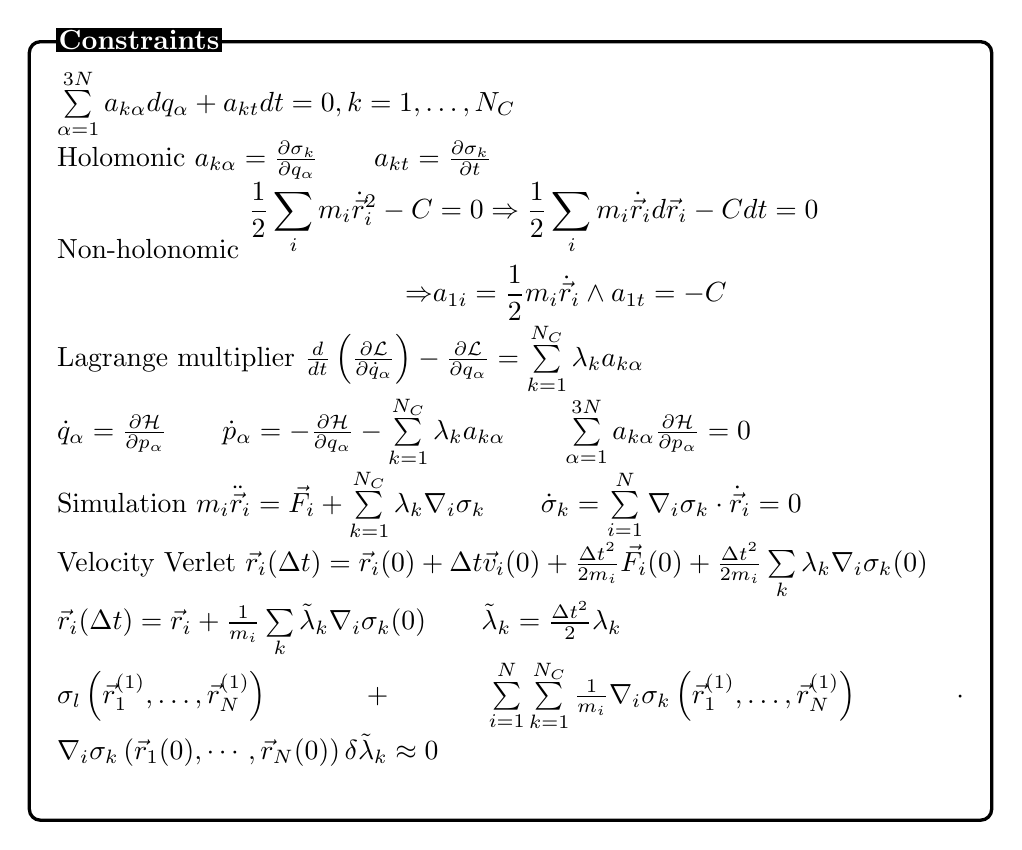
\begin{tikzpicture}
                \node [mybox] (box1){%
                    \begin{minipage}{0.95\textwidth}
                        $\sum\limits_{\alpha=1}^{3N}a_{k\alpha}dq_\alpha + a_{kt}dt = 0, k = 1, \dots, N_C$\\
                        Holomonic $a_{k\alpha} = \frac{\partial\sigma_k}{\partial q_\alpha}\qquad a_{kt} = \frac{\partial\sigma_k}{\partial t}$\\
                        Non-holonomic $\begin{aligned}\frac{1}{2}\sum\limits_im_i\dot{\vec{r}}_i^2 - C &= 0\Rightarrow \frac{1}{2}\sum\limits_im_i\dot{\vec{r}}_id\vec{r}_i -Cdt = 0\\\Rightarrow &a_{1i} = \frac{1}{2}m_i\dot{\vec{r}}_i\land a_{1t} = -C\end{aligned}$\\
                        Lagrange multiplier $\frac{d}{dt}\left(\frac{\partial\mathcal{L}}{\partial\dot{q}_\alpha}\right)-\frac{\partial\mathcal{L}}{\partial q_\alpha} = \sum\limits_{k=1}^{N_C}\lambda_ka_{k\alpha}$\\
                        $\dot{q}_\alpha = \frac{\partial\mathcal{H}}{\partial p_\alpha}\qquad \dot{p}_\alpha = -\frac{\partial\mathcal{H}}{\partial q_\alpha}-\sum\limits_{k=1}^{N_C}\lambda_ka_{k\alpha}\qquad\sum\limits_{\alpha=1}^{3N}a_{k\alpha}\frac{\partial\mathcal{H}}{\partial p_\alpha}=0$\\
                        Simulation $m_i\ddot{\vec{r}}_i = \vec{F}_i + \sum\limits_{k=1}^{N_C}\lambda_k\nabla_i\sigma_k\qquad \dot{\sigma}_k = \sum\limits_{i=1}^{N}\nabla_i\sigma_k\cdot\dot{\vec{r}}_i=0$\\
                        Velocity Verlet $\vec{r}_i(\Delta t) = \vec{r}_i(0) + \Delta t\vec{v}_i(0) + \frac{\Delta t^2}{2m_i}\vec{F}_i(0)+\frac{\Delta t^2}{2m_i}\sum\limits_k\lambda_k\nabla_i\sigma_k(0)$\\
                        $\vec{r}_i(\Delta t) = \vec{r}_i + \frac{1}{m_i}\sum\limits_{k}\tilde{\lambda}_k\nabla_i\sigma_k(0)\qquad \tilde{\lambda}_k = \frac{\Delta t^2}{2}\lambda_k$\\
                        $\sigma_l\left(\vec{r}_1^{(1)},\dots, \vec{r}_N^{(1)}\right)+\sum\limits_{i=1}^N\sum\limits_{k=1}^{N_C}\frac{1}{m_i}\nabla_i\sigma_k\left(\vec{r}_1^{(1)},\dots, \vec{r}_N^{(1)}\right)\cdot\nabla_i\sigma_k\left(\vec{r}_1(0),\cdots,\vec{r}_N(0)\right)\delta\tilde{\lambda}_k\approx0$\\
                    \end{minipage}
                };
                \node[fancytitle, inner sep = 1pt, right=10pt] at (box1.north west) {Constraints};
            \end{tikzpicture}
        \end{minipage}
    };
    \node[fancytitle, right=10pt] at (box.north west) {Introduction to molecular dynamics (contd)};
\end{tikzpicture}
\begin{tikzpicture}
    \node [mybox] (box){%
        \begin{minipage}{0.233\textwidth}
            \begin{tikzpicture}
                \node [mybox] (box1){%
                    \begin{minipage}{0.95\textwidth}
                        Computable on $a:\frac{da}{dt} = \{a,\mathcal{H}\}$\\
                        $iL = \sum\limits_\alpha\left[\frac{\partial\mathcal{H}}{\partial q_\alpha}\frac{\partial}{\partial q_\alpha}-\frac{\partial\mathcal{H}}{\partial q_\alpha}\frac{\partial}{\partial p_\alpha}\right]\Rightarrow iLa = \{a, \mathcal{H}\}\Rightarrow\frac{da}{dt} = iLa\Rightarrow a(x_t) = e^{iLt}a(x_0)$\\
                        Split $iL_1 = \sum\limits_\alpha\frac{\partial\mathcal{H}}{\partial p_\alpha}\frac{\partial}{\partial q_\alpha}\qquad iL_2 = -\sum\limits_\alpha\frac{\partial\mathcal{H}}{\partial q_\alpha}\frac{\partial}{\partial p_\alpha}$\\
                        $iL_1iL_2\phi(x)\neq iL_2iL_1\phi(x)\Rightarrow iL_1iL_2-iL_2iL_1 \equiv[iL_1,iL_2]\neq 0$\\
                    \end{minipage}
                };
                \node[fancytitle, inner sep = 1pt, right=10pt] at (box1.north west) {Liouville operator};
            \end{tikzpicture}
            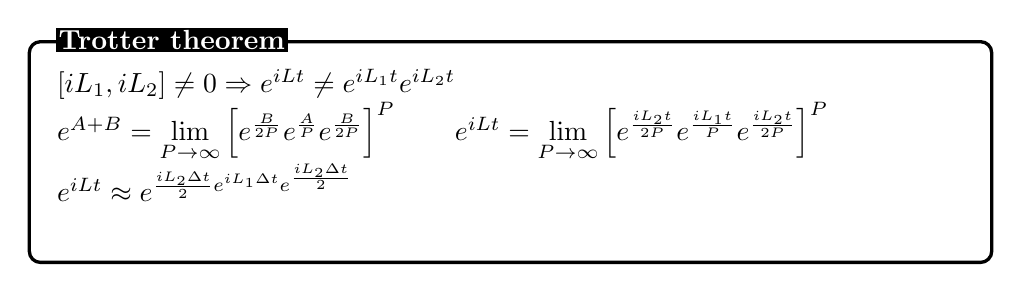
\begin{tikzpicture}
                \node [mybox] (box1){%
                    \begin{minipage}{0.95\textwidth}
                        $[iL_1, iL_2]\neq 0\Rightarrow e^{iLt}\neq e^{iL_1t}e^{iL_2t}$\\
                        $e^{A+B} = \lim\limits_{P\rightarrow\infty}\left[e^{\frac{B}{2P}}e^{\frac{A}{P}}e^{\frac{B}{2P}}\right]^P \qquad e^{iLt} = \lim\limits_{P\rightarrow\infty}\left[e^{\frac{iL_2t}{2P}}e^{\frac{iL_1t}{P}}e^{\frac{iL_2t}{2P}}\right]^P$\\
                        $e^{iLt}\approx e^{\frac{iL_2\Delta t}{2}e^{iL_1\Delta t}e^{\frac{iL_2\Delta t}{2}}}$\\
                    \end{minipage}
                };
                \node[fancytitle, inner sep = 1pt, right=10pt] at (box1.north west) {Trotter theorem};
            \end{tikzpicture}
            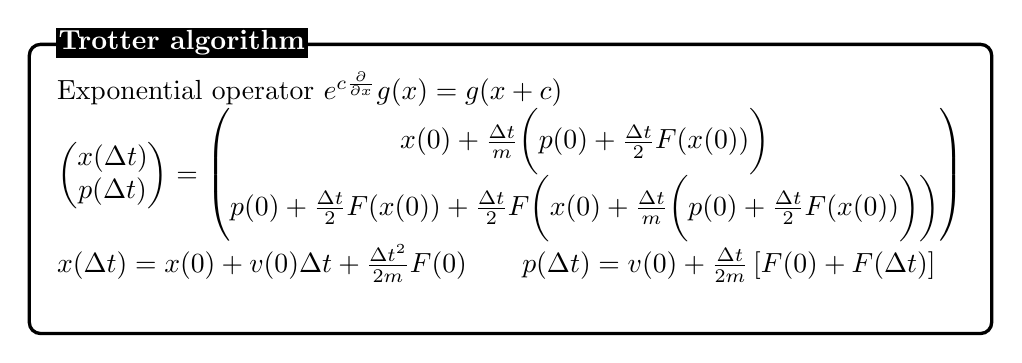
\begin{tikzpicture}
                \node [mybox] (box1){%
                    \begin{minipage}{0.95\textwidth}
                        Exponential operator $e^{c\frac{\partial}{\partial x}}g(x) = g(x+c)$\\
                        $\begin{pmatrix} x(\Delta t)\\ p(\Delta t)\end{pmatrix} = \begin{pmatrix} x(0) + \frac{\Delta t}{m}\biggl(p(0) + \frac{\Delta t}{2}F(x(0))\biggr) \\ p(0) + \frac{\Delta t}{2}F(x(0)) + \frac{\Delta t}{2}F\biggl(x(0) + \frac{\Delta t}{m}\biggl(p(0) + \frac{\Delta t}{2}F(x(0))\biggr)\biggr)\end{pmatrix}$
                        $x(\Delta t) = x(0) + v(0) \Delta t + \frac{\Delta t^2}{2m}F(0)\qquad p(\Delta t) = v(0) + \frac{\Delta t}{2m}\left[ F(0) + F(\Delta t)\right]$\\

                    \end{minipage}
                };
                \node[fancytitle, inner sep = 1pt, right=10pt] at (box1.north west) {Trotter algorithm};
            \end{tikzpicture}
            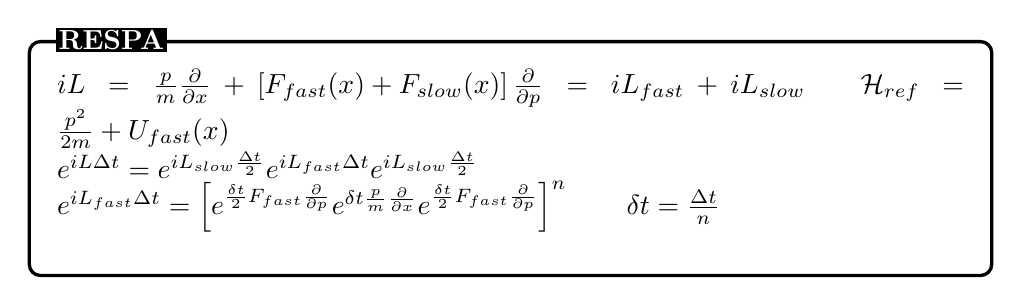
\begin{tikzpicture}
                \node [mybox] (box1){%
                    \begin{minipage}{0.95\textwidth}
                        $iL = \frac{p}{m}\frac{\partial}{\partial x} + \left[F_{fast}(x) + F_{slow}(x)\right]\frac{\partial}{\partial p} = iL_{fast} + iL_{slow}\qquad \mathcal{H}_{ref} = \frac{p^2}{2m} + U_{fast}(x)$\\
                        $e^{iL\Delta t} = e^{iL_{slow}\frac{\Delta t}{2}}e^{iL_{fast}\Delta t}e^{iL_{slow}\frac{\Delta t}{2}}$\\
                        $e^{iL_{fast}\Delta t} = \left[e^{\frac{\delta t}{2}F_{fast}\frac{\partial}{\partial p}}e^{\delta t\frac{p}{m}\frac{\partial}{\partial x}}e^{\frac{\delta t}{2}F_{fast}\frac{\partial}{\partial p}}\right]^n\qquad \delta t = \frac{\Delta t}{n}$\\

                    \end{minipage}
                };
                \node[fancytitle, inner sep = 1pt, right=10pt] at (box1.north west) {RESPA};
            \end{tikzpicture}
        \end{minipage}
    };
    \node[fancytitle, right=10pt] at (box.north west) {Direct translation};
\end{tikzpicture}
\begin{tikzpicture}
    \node [mybox] (box){%
        \begin{minipage}{0.233\textwidth}
            \begin{tikzpicture}
                \node [mybox] (box1){%
                    \begin{minipage}{0.95\textwidth}
                        Non bonded interaction $U_{nb}(\vec{r}_1, \dots, \vec{r}_N) = \sum\limits_{i<j\in nb}\left\{4\epsilon_{ij}\left[\left(\frac{\sigma_{ij}}{r_{ij}}\right)^{12}-\left(\frac{\sigma_{ij}}{r_{ij}}\right)^6\right]+\frac{q_iq_j}{r_{ij}}\right\}$\\
                        Error function $erf(x) = \frac{2}{\sqrt{\pi}}\int_0^x e^{-t^2}dt\qquad\lim\limits_{x\to\infty}erf(x) = 1\qquad erf(0) = 0$\\
                        Complement error $erfc(x) = 1-erf(x) = \frac{2}{\sqrt{\pi}}\int_x^\infty e^{-t^2}dt\qquad\lim\limits_{x\to\infty}erf(x) = 0\qquad erf(0) = 1$\\
                        $\frac{1}{r} = \frac{\overbrace{erfc(\alpha r)}^{\text{short-ranged}}}{r} + \frac{\overbrace{erf(\alpha r)}^{\text{long-ranged}}}{r}\qquad U_{nb} = U_{short} + U_{long}\qquad \vec{r}_{ij} = |\vec{r}_i-\vec{r}_j + \vec{S}|\qquad \vec{S} = \vec{m}L$\\
                        $U_{short}(\vec{r}_1, \dots, \vec{r}_N) = \sum\limits_{\vec{S}}\sum\limits_{i>j\in nb}\left\{4\epsilon_{ij}\left[\left(\frac{\sigma_{ij}}{r_{ij,\vec{S}}}\right)^{12} - \left(\frac{\sigma_{ij}}{r_{ij, \vec{S}}}\right)^6\right]+\frac{q_iq_jerfc(\alpha r_{ij, \vec{S}})}{r_{ij, \vec{S}}}\right\}$\\
                        $U_{long}(\vec{r}_1, \dots, \vec{r}_N) = \sum\limits_{\vec{S}}\sum\limits_{i>h\in nb}\frac{q_iq_jerf(\alpha r_{ij, \vec{S}})}{r_{ij, \vec{S}}}$\\
                    \end{minipage}
                };
                \node[fancytitle, inner sep = 1pt, right=10pt] at (box1.north west) {Periodic boundary condition};
            \end{tikzpicture}
            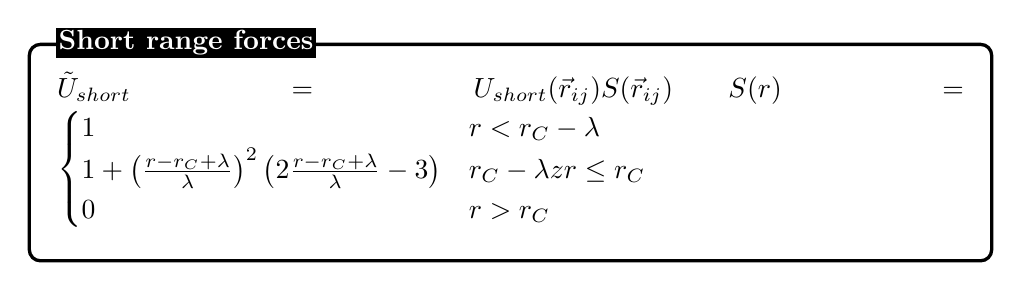
\begin{tikzpicture}
                \node [mybox] (box1){%
                    \begin{minipage}{0.95\textwidth}
                        $\tilde{U}_{short} = U_{short}(\vec{r}_{ij})S(\vec{r}_{ij})\qquad S(r) = \begin{cases} 1 & r < r_C-\lambda\\1+\left(\frac{r-r_C+\lambda}{\lambda}\right)^2\left(2\frac{r-r_C+\lambda}{\lambda}-3\right) &r_C-\lambda z r \le r_C\\0 & r>r_C\end{cases}$\\
                    \end{minipage}
                };
                \node[fancytitle, inner sep = 1pt, right=10pt] at (box1.north west) {Short range forces};
            \end{tikzpicture}
        \end{minipage}
    };
    \node[fancytitle, right=10pt] at (box.north west) {Evaluation of energy and forces};
\end{tikzpicture}
\begin{tikzpicture}
    \node [mybox] (box){%
        \begin{minipage}{0.233\textwidth}
            \begin{tikzpicture}
                \node [mybox] (box1){%
                    \begin{minipage}{0.95\textwidth}
                        $C_{\vec{g}} = \frac{4\pi}{|\vec{g}|^2}e^{-\frac{|\vec{g}|^2}{4\alpha^2}}\qquad \frac{1}{V}\sum\limits_{\vec{g}}C_{\vec{g}}e^{i\vec{g}\cdot\vec{r}} = \frac{1}{V}\sum\limits_{i\neq j}q_iq_j\sum\limits_{\vec{g}\in\mathcal{S}}\frac{4\pi}{|\vec{g}|^2}e^{-\frac{|\vec{g}|^2}{2\alpha^2}}e^{i\vec{g}\cdot(\vec{r}_i-\vec{r}_j)}$\\
                        $U_{long} = \frac{1}{V}\sum\limits_{i,j}q_iq_j\sum\limits_{\vec{g}\in\mathcal{S}}\frac{4\pi}{|\vec{g}|^2}e^{-\frac{|\vec{g}|^2}{4\alpha^2}}e^{i\vec{g}\cdot(\vec{r}_i-\vec{r}_j)}-\frac{1}{V}\sum\limits_{i}q_i^2\sum\limits_{\vec{g}\in\mathcal{S}}\frac{4\pi}{|\vec{g}|^2}e^{-\frac{|\vec{g}|^2}{4\alpha^2}}$\\
                        $U_{long} = \frac{1}{V}\sum\limits_{\vec{g}\in\mathcal{S}}\frac{4\pi}{|\vec{g}|^2}e^{-\frac{|\vec{g}|^2}{4\alpha^2}}|S(\vec{g})|^2-\frac{\alpha}{\sqrt{\pi}}\sum\limits_i q_i^2$\\
                    \end{minipage}
                };
                \node[fancytitle, inner sep = 1pt, right=10pt] at (box1.north west) {Long range forces};
            \end{tikzpicture}
            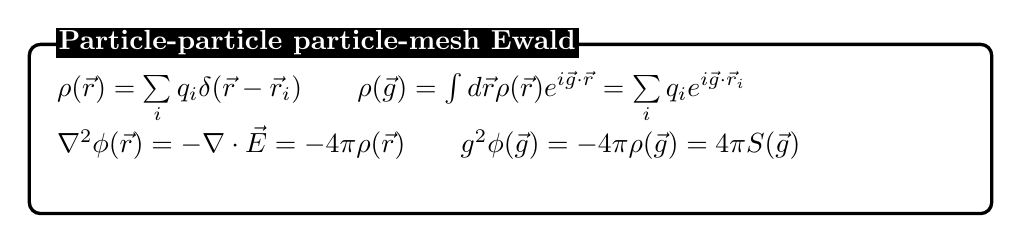
\begin{tikzpicture}
                \node [mybox] (box1){%
                    \begin{minipage}{0.95\textwidth}
                        $\rho(\vec{r})= \sum\limits_iq_i\delta(\vec{r}-\vec{r}_i)\qquad \rho(\vec{g}) = \int d\vec{r}\rho(\vec{r})e^{i\vec{g}\cdot\vec{r}} = \sum\limits_i q_ie^{i\vec{g}\cdot\vec{r}_i}$\\
                        $\nabla^2\phi(\vec{r}) = -\nabla\cdot\vec{E}=-4\pi\rho(\vec{r})\qquad g^2\phi(\vec{g}) = -4\pi\rho(\vec{g})= 4\pi S(\vec{g})$\\
                    \end{minipage}
                };
                \node[fancytitle, inner sep = 1pt, right=10pt] at (box1.north west) {Particle-particle particle-mesh Ewald};
            \end{tikzpicture}
        \end{minipage}
    };
    \node[fancytitle, right=10pt] at (box.north west) {Evaluation of energy and forces (contd)};
\end{tikzpicture}
\begin{tikzpicture}
    \node [mybox] (box){%
        \begin{minipage}{0.233\textwidth}
            \begin{tikzpicture}
                \node [mybox] (box1){%
                    \begin{minipage}{0.95\textwidth}
                        Helmholtz free energy $A(N, V, T) = E(N, V, T) -TS(N, V, T)$\\
                        $dA = SdT-PdV+\mu dN\qquad S = -\left(\frac{\partial A}{\partial T}\right)_{N, V}\qquad P = -\left(\frac{\partial A}{\partial V}\right)_{N, T}\qquad \mu = \left(\frac{\partial A}{\partial N}\right)_{V, T}$\\
                    \end{minipage}
                };
                \node[fancytitle, inner sep = 1pt, right=10pt] at (box1.north west) {Thermodynamics};
            \end{tikzpicture}
            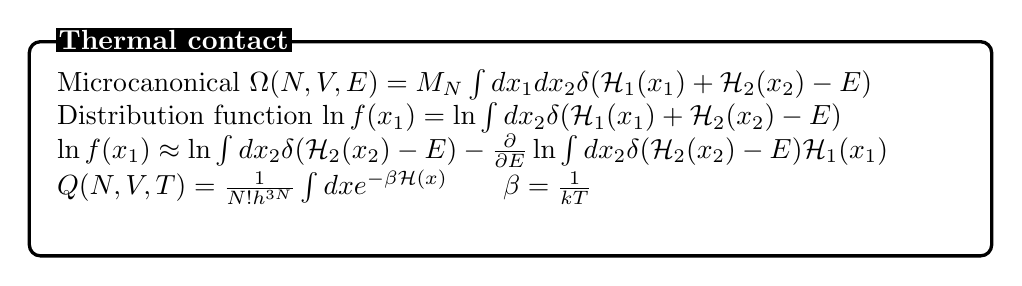
\begin{tikzpicture}
                \node [mybox] (box1){%
                    \begin{minipage}{0.95\textwidth}
                        Microcanonical $\Omega(N, V, E) = M_N\int dx_1dx_2\delta(\mathcal{H}_1(x_1)+\mathcal{H}_2(x_2)-E)$\\
                        Distribution function $\ln f(x_1) = \ln\int dx_2\delta(\mathcal{H}_1(x_1)+\mathcal{H}_2(x_2)-E)$\\
                        $\ln f(x_1)\approx \ln\int dx_2\delta(\mathcal{H}_2(x_2)-E)-\frac{\partial}{\partial E}\ln\int dx_2\delta(\mathcal{H}_2(x_2)-E)\mathcal{H}_1(x_1)$\\
                        $Q(N, V, T) = \frac{1}{N!h^{3N}}\int dxe^{-\beta\mathcal{H}(x)}\qquad \beta = \frac{1}{kT}$\\
                    \end{minipage}
                };
                \node[fancytitle, inner sep = 1pt, right=10pt] at (box1.north west) {Thermal contact};
            \end{tikzpicture}
            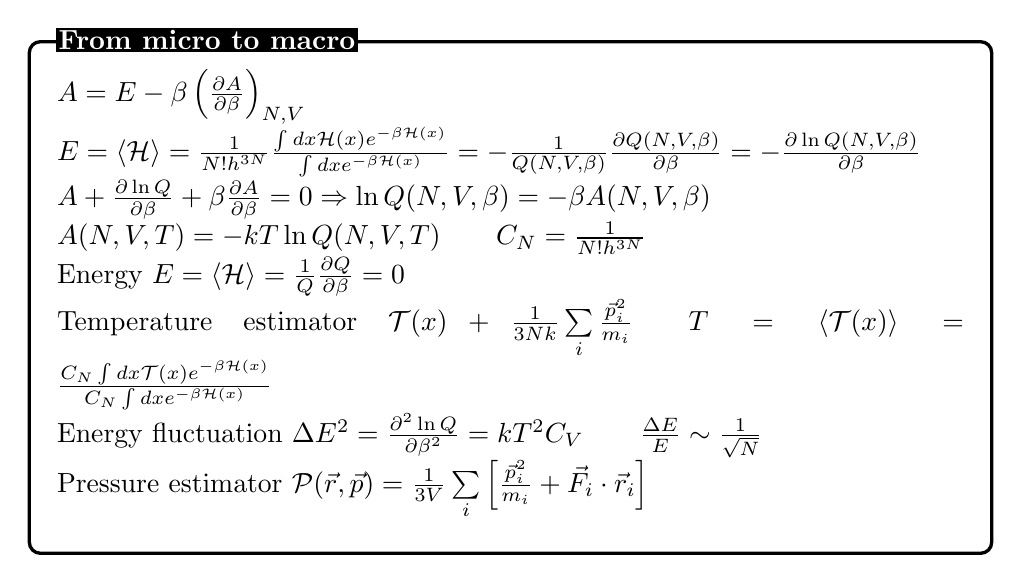
\begin{tikzpicture}
                \node [mybox] (box1){%
                    \begin{minipage}{0.95\textwidth}
                        $A = E-\beta\left(\frac{\partial A}{\partial \beta}\right)_{N,V}$\\
                        $E = \langle\mathcal{H}\rangle = \frac{1}{N!h^{3N}}\frac{\int dx\mathcal{H}(x)e^{-\beta\mathcal{H}(x)}}{\int dxe^{-\beta\mathcal{H}(x)}}=-\frac{1}{Q(N, V, \beta)}\frac{\partial Q(N, V, \beta)}{\partial\beta} = -\frac{\partial\ln Q(N, V, \beta)}{\partial\beta}$\\
                        $A + \frac{\partial\ln Q}{\partial\beta} + \beta\frac{\partial A}{\partial \beta} = 0\Rightarrow \ln Q(N, V, \beta) = -\beta A(N, V, \beta)$\\
                        $A(N, V, T) = -kT\ln Q(N, V, T)\qquad C_N = \frac{1}{N!h^{3N}}$\\
                        Energy $E = \langle\mathcal{H}\rangle = \frac{1}{Q}\frac{\partial Q}{\partial\beta} = 0$\\
                        Temperature estimator $\mathcal{T}(x) + \frac{1}{3Nk}\sum\limits_i\frac{\vec{p}_i^2}{m_i}\qquad T = \langle\mathcal{T}(x)\rangle = \frac{C_N\int dx\mathcal{T}(x)e^{-\beta\mathcal{H}(x)}}{C_N\int dx e^{-\beta\mathcal{H}(x)}}$\\
                        Energy fluctuation $\Delta E^2 = \frac{\partial^2 \ln Q}{\partial \beta^2} = kT^2C_V\qquad \frac{\Delta E}{E} \sim \frac{1}{\sqrt{N}}$\\
                        Pressure estimator $\mathcal{P}(\vec{r}, \vec{p}) = \frac{1}{3V}\sum\limits_i\left[\frac{\vec{p}_i^2}{m_i} + \vec{F}_i\cdot\vec{r}_i\right]$\\
                    \end{minipage}
                };
                \node[fancytitle, inner sep = 1pt, right=10pt] at (box1.north west) {From micro to macro};
            \end{tikzpicture}
        \end{minipage}
    };
    \node[fancytitle, inner sep = 1pt, right=10pt] at (box.north west) {Canonical ensemble};
\end{tikzpicture}
\begin{tikzpicture}
    \node [mybox] (box){%
        \begin{minipage}{0.233\textwidth}
            \begin{tikzpicture}
                \node [mybox] (box1){%
                    \begin{minipage}{0.95\textwidth}
                        $\bar{K} = \frac{N_j}{2\beta}\qquad K = \frac{1}{2}\sum\limits_{i}m_i\vec{v}_i^2\qquad\vec{v}_i\to\frac{\vec{v}_i}{\alpha}\qquad \alpha = \sqrt{\frac{\bar{K}}{K}}$\\
                        $\bar{K} = \frac{1}{2}\sum\limits_{i}m_i\frac{\vec{v}_i^2}{\alpha^2} = \frac{\bar{K}}{2K}\sum\limits_{i}m_i\vec{v}_i^2$\\
                    \end{minipage}
                };
                \node[fancytitle, inner sep = 1pt, right=10pt] at (box1.north west) {Velocity rescaling};
            \end{tikzpicture}
            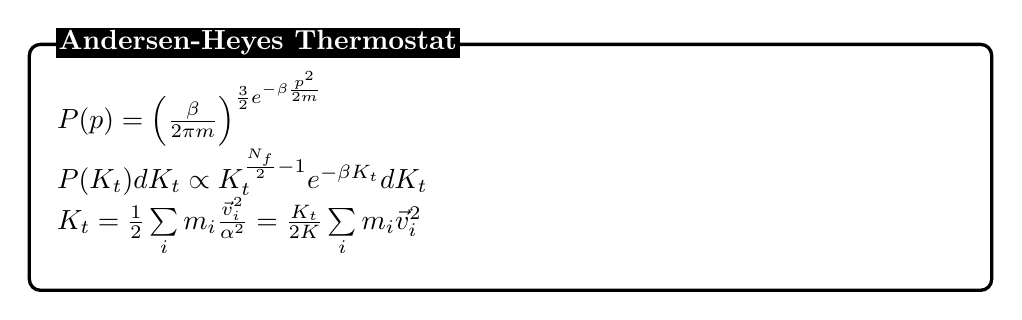
\begin{tikzpicture}
                \node [mybox] (box1){%
                    \begin{minipage}{0.95\textwidth}
                        $P(p) = \left(\frac{\beta}{2\pi m}\right)^{\frac{3}{2}e^{-\beta\frac{p^2}{2m}}}$\\
                        $P(K_t)dK_t\propto K_t^{\frac{N_f}{2}-1}e^{-\beta K_t}dK_t$\\
                        $K_t = \frac{1}{2}\sum\limits_{i}m_i\frac{\vec{v}_i^2}{\alpha^2} = \frac{K_t}{2K}\sum\limits_{i}m_i\vec{v}_i^2$\\
                    \end{minipage}
                };
                \node[fancytitle, inner sep = 1pt, right=10pt] at (box1.north west) {Andersen-Heyes Thermostat};
            \end{tikzpicture}
            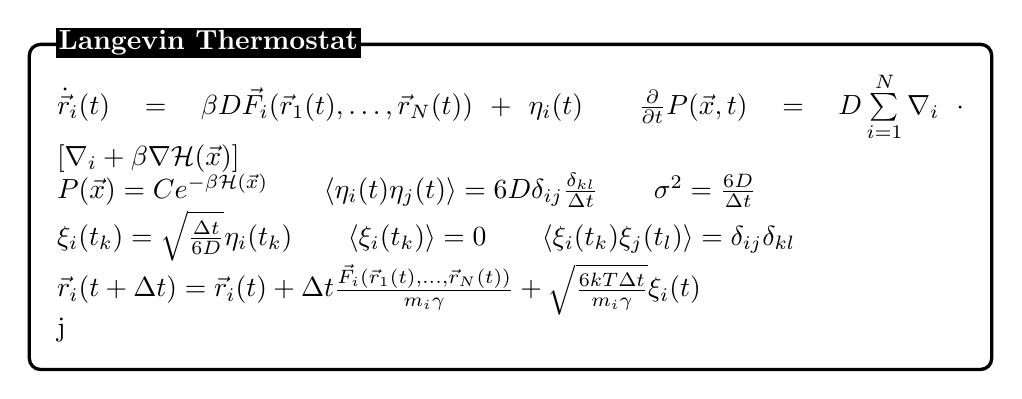
\begin{tikzpicture}
                \node [mybox] (box1){%
                    \begin{minipage}{0.95\textwidth}
                        $\dot{\vec{r}}_i(t) = \beta D\vec{F}_i(\vec{r}_1(t), \dots, \vec{r}_N(t)) + \eta_i(t)\qquad\frac{\partial}{\partial t}P(\vec{x}, t) = D\sum\limits_{i=1}^N\nabla_i\cdot\left[\nabla_i + \beta\nabla\mathcal{H}(\vec{x})\right]$\\
                        $P(\vec{x}) = Ce^{-\beta\mathcal{H}(\vec{x})}\qquad\langle\eta_i(t)\eta_j(t)\rangle = 6 D\delta_{ij}\frac{\delta_{kl}}{\Delta t}\qquad \sigma^2 = \frac{6D}{\Delta t}$\\
                        $\xi_i(t_k) = \sqrt{\frac{\Delta t}{6D}}\eta_i(t_k)\qquad\langle\xi_i(t_k)\rangle = 0\qquad \langle\xi_i(t_k)\xi_j(t_l)\rangle = \delta_{ij}\delta_{kl} $\\
                        $\vec{r}_i(t+\Delta t) = \vec{r}_i(t) +\Delta t\frac{\vec{F}_i(\vec{r}_1(t), \dots, \vec{r}_N(t))}{m_i\gamma} + \sqrt{\frac{6kT\Delta t}{m_i\gamma}}\xi_i(t)$\\j
                    \end{minipage}
                };
                \node[fancytitle, inner sep = 1pt, right=10pt] at (box1.north west) {Langevin Thermostat};
            \end{tikzpicture}
            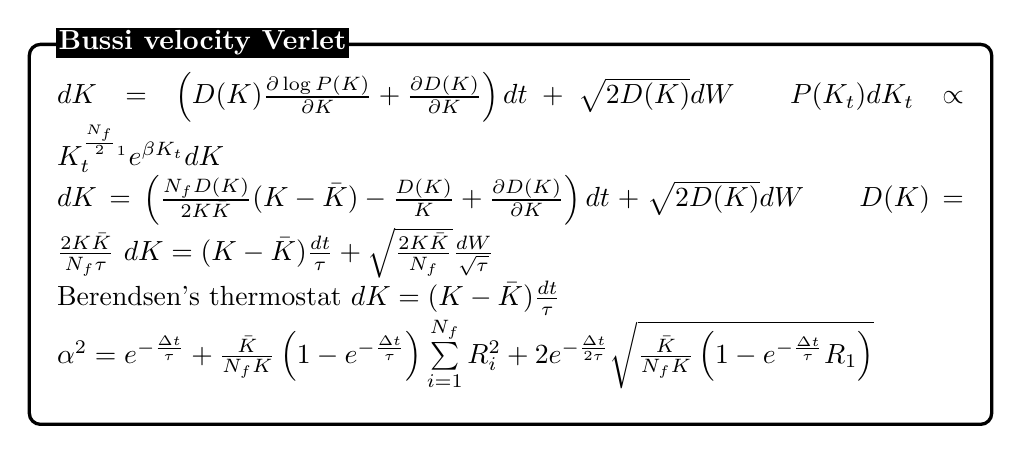
\begin{tikzpicture}
                \node [mybox] (box1){%
                    \begin{minipage}{0.95\textwidth}
                        $dK = \left(D(K)\frac{\partial\log P(K)}{\partial K}+\frac{\partial D(K)}{\partial K}\right)dt + \sqrt{2D(K)}dW\qquad P(K_t)dK_t\propto K_t^{\frac{N_f}{2}_1}e^{\beta K_t}dK$\\
                        $dK = \left(\frac{N_f D(K)}{2K\bar{K}}(K-\bar{K})-\frac{D(K)}{K}+\frac{\partial D(K)}{\partial K}\right)dt + \sqrt{2D(K)}dW\qquad D(K) = \frac{2K\bar{K}}{N_f\tau}$
                        $dK = (K-\bar{K})\frac{dt}{\tau} + \sqrt{\frac{2K\bar{K}}{N_f}}\frac{dW}{\sqrt{\tau}}$\\
                        Berendsen's thermostat $dK = (K-\bar{K})\frac{dt}{\tau}$\\
                        $\alpha^2 = e^{-\frac{\Delta t}{\tau}} + \frac{\bar{K}}{N_f K}\left(1-e^{-\frac{\Delta t}{\tau}}\right)\sum\limits_{i=1}^{N_f}R_i^2+2e^{-\frac{\Delta t}{2\tau}}\sqrt{\frac{\bar{K}}{N_f K}\left(1-e^{-\frac{\Delta t}{\tau}}R_1\right)}$\\
                    \end{minipage}
                };
                \node[fancytitle, inner sep = 1pt, right=10pt] at (box1.north west) {Bussi velocity Verlet};
            \end{tikzpicture}
            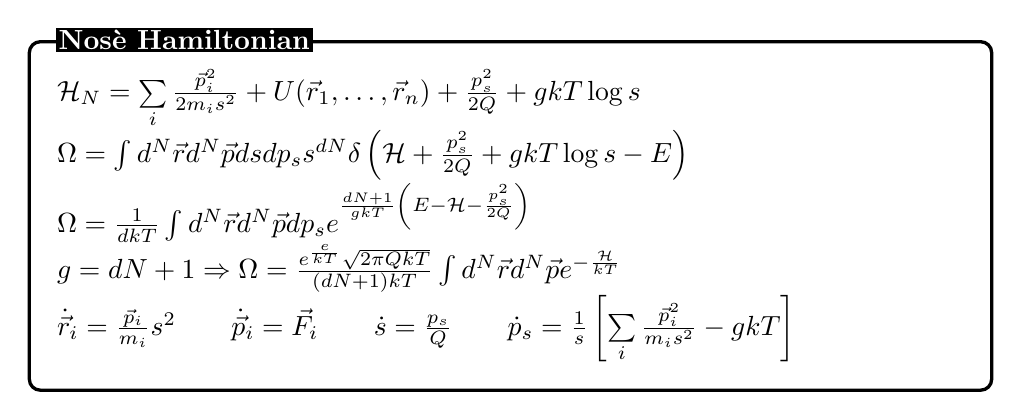
\begin{tikzpicture}
                \node [mybox] (box1){%
                    \begin{minipage}{0.95\textwidth}
                        $\mathcal{H}_N = \sum\limits_{i}\frac{\vec{p}_i^2}{2m_is^2} + U(\vec{r}_1, \dots, \vec{r}_n)+\frac{p_s^2}{2Q} + gkT\log s$\\
                        $\Omega = \int d^N\vec{r}d^N\vec{p}dsdp_ss^{dN}\delta\left(\mathcal{H} + \frac{p_s^2}{2Q} + gkT\log s - E\right)$\\
                        $\Omega = \frac{1}{dkT}\int d^N\vec{r}d^N\vec{p}dp_se^{\frac{dN+1}{gkT}\left(E-\mathcal{H}-\frac{p_s^2}{2Q}\right)}$\\\
                        $g = dN + 1 \Rightarrow \Omega  = \frac{e^{\frac{e}{kT}}\sqrt{2\pi QkT}}{(dN+1)kT}\int d^N\vec{r}d^N\vec{p}e^{-\frac{\mathcal{H}}{kT}}$\\
                        $\dot{\vec{r}}_i = \frac{\vec{p}_i}{m_i}s^2\qquad \dot{\vec{p}}_i = \vec{F}_i\qquad \dot{s} = \frac{p_s}{Q}\qquad \dot{p}_s = \frac{1}{s}\left[\sum\limits_{i}\frac{\vec{p}_i^2}{m_is^2}-gkT\right]$
                    \end{minipage}
                };
                \node[fancytitle, inner sep = 1pt, right=10pt] at (box1.north west) {Nos\`e Hamiltonian};
            \end{tikzpicture}
        \end{minipage}
    };
    \node[fancytitle, inner sep = 1pt, right=10pt] at (box.north west) {Thermostats};
\end{tikzpicture}
\begin{tikzpicture}
    \node [mybox] (box){%
        \begin{minipage}{0.233\textwidth}
            \begin{tikzpicture}
                \node [mybox] (box1){%
                    \begin{minipage}{0.95\textwidth}
                        $\vec{p}'_i = \frac{\vec{p}_i}{s}\qquad \vec{p}'_s = \frac{p_s}{s}\qquad dt' = \frac{dt}{s}\qquad \frac{d\vec{r}_i}{dt'} = \frac{\vec{p}'_i}{m_i}\qquad\frac{d\vec{p}'_i}{dt'} =\vec{F}_i -\frac{sp'_s}{Q}\vec{p}'_i$\\
                        $\frac{ds}{dt'} = \frac{s^2p_s'}{Q}\qquad \frac{dp'_s}{dt'} = \frac{1}{2}\left[\sum\limits_{i}\frac{(\vec{p}'_i)^2}{m_i}-gkT\right]^2 - \frac{s(p'_s)^2}{Q}\qquad \frac{1}{2}\frac{ds}{dt'} = \frac{d\eta}{dt'}\qquad p_s = p_\eta = sp'_s$\\
                        $\dot{\vec{r}}_i = \frac{\vec{p}_i}{m_i}\qquad \dot{\vec{p}}_i = \vec{F}_i - \frac{P_\eta}{Q}\vec{p}_i\qquad\dot{\eta} = \frac{p_\eta}{Q}\qquad \dot{p}_\eta = \sum\limits_i\frac{\vec{p}_i^2}{m_i} - dNkT$\\
                    \end{minipage}
                };
                \node[fancytitle, inner sep = 1pt, right=10pt] at (box1.north west) {Nos\`e-Hoover equations};
            \end{tikzpicture}
            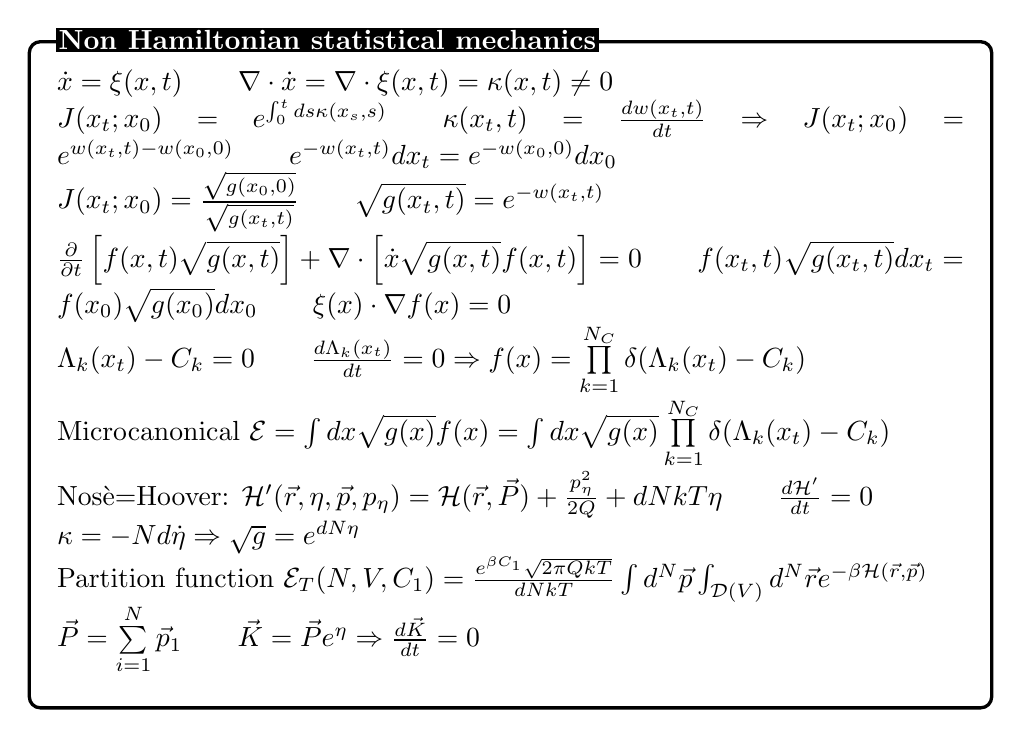
\begin{tikzpicture}
                \node [mybox] (box1){%
                    \begin{minipage}{0.95\textwidth}
                        $\dot{x} = \xi(x, t)\qquad\nabla\cdot\dot{x} = \nabla\cdot\xi(x, t) = \kappa(x,t)\neq 0$\\
                        $J(x_t;x_0) = e^{\int_0^tds\kappa(x_s, s)}\qquad \kappa(x_t, t) = \frac{dw(x_t, t)}{dt}\Rightarrow J(x_t;x_0) = e^{w(x_t, t)-w(x_0, 0)}\qquad e^{-w(x_t, t)}dx_t = e^{-w(x_0, 0)}dx_0$\\
                        $J(x_t;x_0) = \frac{\sqrt{g(x_0,0)}}{\sqrt{g(x_t,t)}}\qquad \sqrt{g(x_t,t)} = e^{-w(x_t,t)}$\\
                        $\frac{\partial}{\partial t}\left[f(x,t)\sqrt{g(x,t)}\right]+\nabla\cdot\left[\dot{x}\sqrt{g(x,t)}f(x,t)\right] = 0\qquad f(x_t, t)\sqrt{g(x_t,t)}dx_t = f(x_0)\sqrt{g(x_0)}dx_0\qquad \xi(x)\cdot\nabla f(x) = 0$\\
                        $\Lambda_k(x_t) -C_k = 0\qquad\frac{d\Lambda_k(x_t)}{dt} = 0\Rightarrow f(x) = \prod\limits_{k=1}^{N_C}\delta(\Lambda_k(x_t)-C_k)$\\
                        Microcanonical $\mathcal{E} = \int dx\sqrt{g(x)}f(x) = \int dx\sqrt{g(x)}\prod\limits_{k=1}^{N_C}\delta(\Lambda_k(x_t)-C_k)$\\
                        Nos\`e=Hoover: $\mathcal{H}'(\vec{r}, \eta, \vec{p}, p_\eta) = \mathcal{H}(\vec{r},\vec{P}) + \frac{p_\eta^2}{2Q} + dNkT\eta\qquad\frac{d\mathcal{H}'}{dt} = 0$\\
                        $\kappa = -Nd\dot{\eta}\Rightarrow \sqrt{g} = e^{dN\eta}$\\
                        Partition function $\mathcal{E}_T(N, V, C_1) = \frac{e^{\beta C_1}\sqrt{2\pi QkT}}{dNkT}\int d^N\vec{p}\int_{\mathcal{D}(V)}d^N\vec{r}e^{-\beta\mathcal{H}(\vec{r}, \vec{p})}$\\
                        $\vec{P} = \sum\limits_{i=1}^N\vec{p}_1\qquad\vec{K} = \vec{P}e^\eta\Rightarrow \frac{d\vec{K}}{dt} = 0$\\
                    \end{minipage}
                };
                \node[fancytitle, inner sep = 1pt, right=10pt] at (box1.north west) {Non Hamiltonian statistical mechanics};
            \end{tikzpicture}
            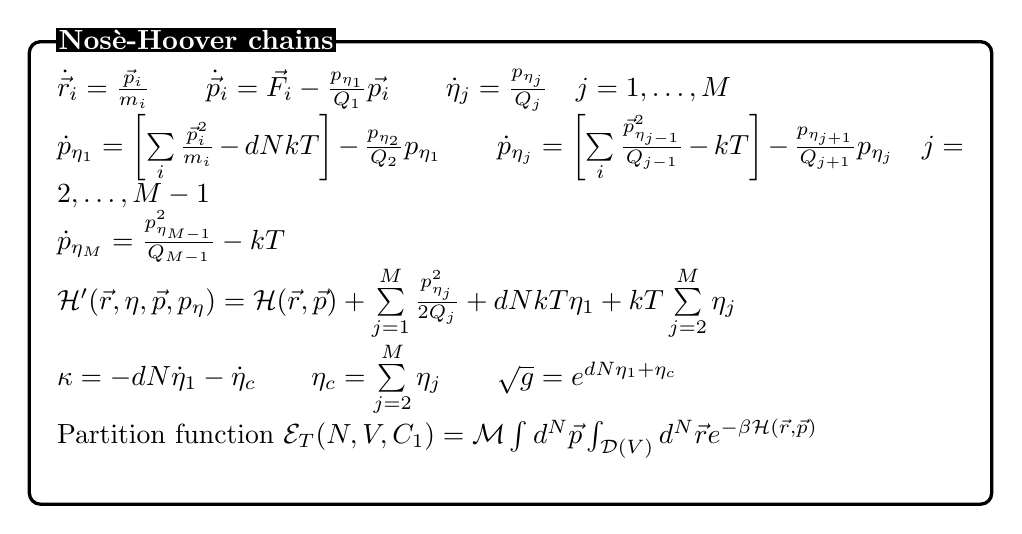
\begin{tikzpicture}
                \node [mybox] (box1){%
                    \begin{minipage}{0.95\textwidth}
			$\dot{\vec{r}}_i = \frac{\vec{p}_i}{m_i}\qquad\dot{\vec{p}}_i = \vec{F}_i - \frac{p_{\eta_1}}{Q_1}\vec{p_i}\qquad\dot{\eta}_j = \frac{p_{\eta_j}}{Q_j}\quad j = 1, \dots, M$\\
                        $\dot{p}_{\eta_1} = \biggl[\sum\limits_i\frac{\vec{p}_i^2}{m_i}-dNkT\biggr] - \frac{p_{\eta_2}}{Q_2}p_{\eta_1}\qquad\dot{p}_{\eta_j} = \biggl[\sum\limits_i\frac{\vec{p}_{\eta_{j-1}}^2}{Q_{j-1}}-kT\biggr] - \frac{p_{\eta_{j+1}}}{Q_{j+1}}p_{\eta_j}\quad j = 2, \dots, M-1$\\
                        $\dot{p}_{\eta_M} = \frac{p^2_{\eta_{M-1}}}{Q_{M-1}}-kT$\\
	                $\mathcal{H}'(\vec{r}, \eta, \vec{p}, p_\eta) = \mathcal{H}(\vec{r}, \vec{p}) + \sum\limits_{j=1}^M\frac{p_{\eta_j}^2}{2Q_j} + dNkT\eta_1 + kT\sum\limits_{j=2}^M\eta_j$\\
                        $\kappa  = -dN\dot{\eta}_1 - \dot{\eta}_c\qquad \eta_c = \sum\limits_{j=2}^M\eta_j\qquad \sqrt{g} = e^{dN\eta_1+\eta_c}$\\
                        Partition function $\mathcal{E}_T(N, V, C_1) = \mathcal{M}\int d^N\vec{p}\int_{\mathcal{D}(V)}d^N\vec{r}e^{-\beta\mathcal{H}(\vec{r}, \vec{p})}$\\
                    \end{minipage}
                };
                \node[fancytitle, inner sep = 1pt, right=10pt] at (box1.north west) {Nos\`e-Hoover chains};
            \end{tikzpicture}
        \end{minipage}
    };
    \node[fancytitle, right=10pt] at (box.north west) {Thermostats (contd)};
\end{tikzpicture}
\begin{tikzpicture}
    \node [mybox] (box){%
        \begin{minipage}{0.233\textwidth}
            \begin{tikzpicture}
                \node [mybox] (box1){%
                    \begin{minipage}{0.95\textwidth}
                        Enthalpy $dH = TdS + \mu dN + VdP\quad T = \left(\frac{\partial H}{\partial S}\right)_{N, P}\quad \langle V\rangle = \left(\frac{\partial H}{\partial P}\right)_{N, S}\quad \mu = \left(\frac{\partial H}{\partial N}\right)_{P, S}$\\
                        Gibbs $dG = \mu dN + VdP - SdT\quad S = -\left(\frac{\partial G}{\partial T}\right)_{N, P}\quad \langle V\rangle = -\left(\frac{\partial G}{\partial P}\right)_{N, T}\quad \mu = -\left(\frac{\partial G}{\partial N}\right)_{P, T}$\\
                    \end{minipage}
                };
                \node[fancytitle, inner sep = 1pt, right=10pt] at (box1.north west) {Legendre transforms};
            \end{tikzpicture}
            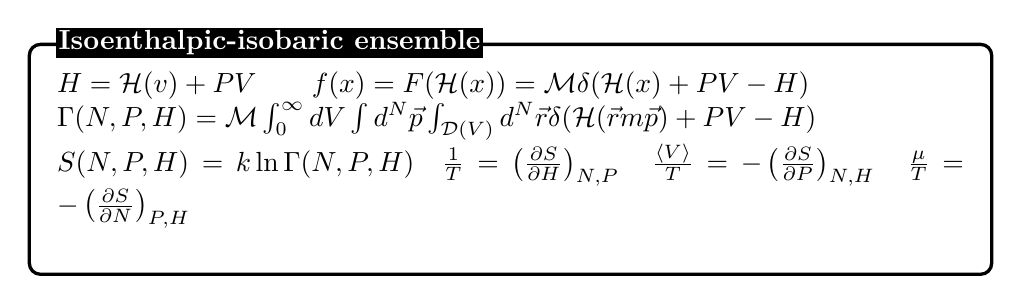
\begin{tikzpicture}
                \node [mybox] (box1){%
                    \begin{minipage}{0.95\textwidth}
                        $H = \mathcal{H}(v) + PV\qquad f(x) = F(\mathcal{H}(x)) = \mathcal{M}\delta(\mathcal{H}(x) +PV -H)$\\
                        $\Gamma(N, P, H) = \mathcal{M}\int_0^\infty dV\int d^N\vec{p}\int_{\mathcal{D}(V)}d^N\vec{r}\delta(\mathcal{H}(\vec{r}m \vec{p}) + PV - H)$\\
                        $S(N, P, H) = k\ln\Gamma(N, P, H)\quad \frac{1}{T} = \left(\frac{\partial S}{\partial H}\right)_{N, P}\quad \frac{\langle V\rangle}{T} = -\left(\frac{\partial S}{\partial P}\right)_{N, H}\quad \frac{\mu}{T} = -\left(\frac{\partial S}{\partial N}\right)_{P, H}$\\
                    \end{minipage}
                };
                \node[fancytitle, inner sep = 1pt, right=10pt] at (box1.north west) {Isoenthalpic-isobaric ensemble};
            \end{tikzpicture}
            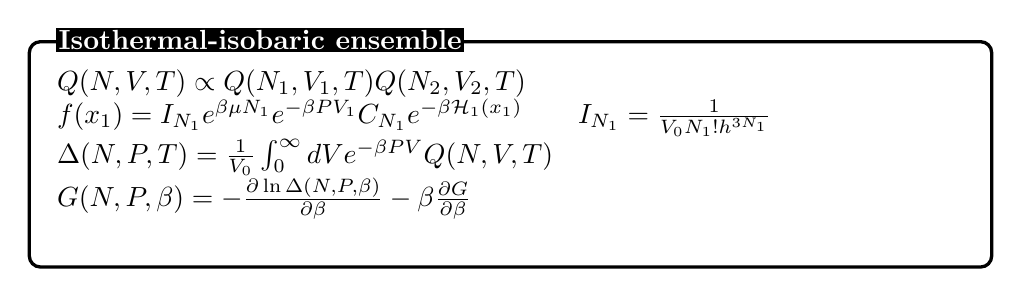
\begin{tikzpicture}
                \node [mybox] (box1){%
                    \begin{minipage}{0.95\textwidth}
                        $Q(N, V, T)\propto Q(N_1, V_1, T)Q(N_2, V_2, T)$\\
                        $f(x_1) = I_{N_1}e^{\beta\mu N_1}e^{-\beta PV_1}C_{N_1}e^{-\beta\mathcal{H}_1(x_1)}\qquad I_{N_1} = \frac{1}{V_0N_1!h^{3N_1}}$\\
                        $\Delta(N, P, T) = \frac{1}{V_0}\int_0^{\infty}dV e^{-\beta PV}Q(N, V, T)$\\
                        $G(N, P, \beta) = -\frac{\partial\ln\Delta(N, P, \beta)}{\partial \beta}-\beta\frac{\partial G}{\partial \beta}$\\
                    \end{minipage}
                };
                \node[fancytitle, inner sep = 1pt, right=10pt] at (box1.north west) {Isothermal-isobaric ensemble};
            \end{tikzpicture}
            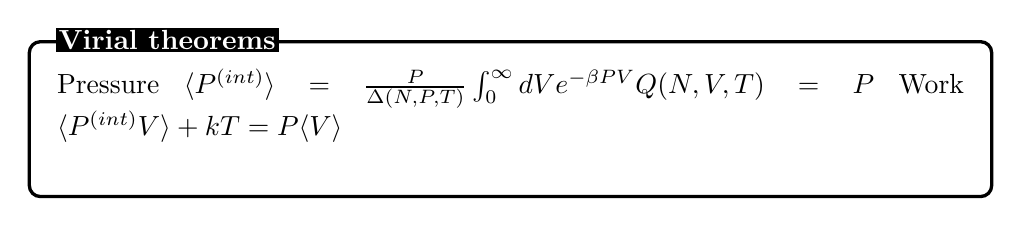
\begin{tikzpicture}
                \node [mybox] (box1){%
                    \begin{minipage}{0.95\textwidth}
                        Pressure $\langle P^{(int)}\rangle = \frac{P}{\Delta(N, P, T)}\int_0^{\infty} dVe^{-\beta PV}Q(N, V, T) = P$
                        Work $\langle P^{(int)}V\rangle + kT = P\langle V\rangle$\\
                    \end{minipage}
                };
                \node[fancytitle, inner sep = 1pt, right=10pt] at (box1.north west) {Virial theorems};
            \end{tikzpicture}
            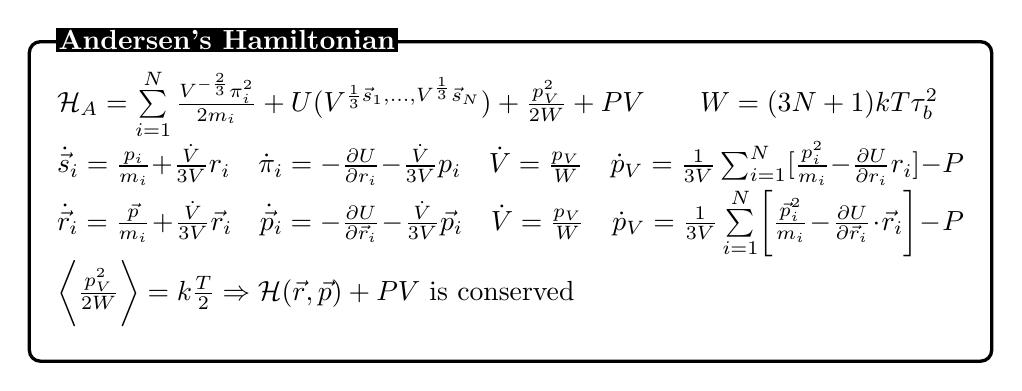
\begin{tikzpicture}
                \node [mybox] (box1){%
                    \begin{minipage}{0.95\textwidth}
                        $\mathcal{H}_A = \sum\limits_{i=1}^N\frac{V^{-\frac{2}{3}}\pi_i^2}{2m_i} + U(V^{\frac{1}{3}\vec{s}_1, \dots, V^{\frac{1}{3}}\vec{s}_N}) + \frac{p^2_V}{2W} + PV\qquad W = (3N+1)kT\tau_b^2$\\
	                $\dot{\vec{s}}_i = \frac{p_i}{m_i} + \frac{\dot{V}}{3V} r_i\quad \dot{\pi}_i = - \frac{\partial U}{\partial r_i} - \frac{\dot{V} }{3V} p_i\quad \dot{V} = \frac{p_V}{W}\quad \dot{p}_V = \frac{1}{3V} \sum^N_{i=1} [\frac{p^2_i}{m_i} - \frac{\partial U}{\partial r_i} r_i] -P$\\
                        $\dot{\vec{r}}_i = \frac{\vec{p}}{m_i} + \frac{\dot{V}}{3V}\vec{r}_i\quad \dot{\vec{p}}_i = -\frac{\partial U}{\partial\vec{r}_i} -\frac{\dot{V}}{3V}\vec{p}_i\quad \dot{V} = \frac{p_V}{W}\quad \dot{p}_V = \frac{1}{3V}\sum\limits_{i=1}^N\biggl[\frac{\vec{p}_i^2}{m_i}-\frac{\partial U}{\partial\vec{r}_i}\cdot\vec{r}_i\biggr]-P$\\
	                $\biggl\langle\frac{p_V^2}{2W}\biggr\rangle = k\frac{T}{2}\Rightarrow \mathcal{H}(\vec{r},\vec{p}) + PV\text{ is conserved}$\\
                    \end{minipage}
                };
                \node[fancytitle, inner sep = 1pt, right=10pt] at (box1.north west) {Andersen's Hamiltonian};
            \end{tikzpicture}
            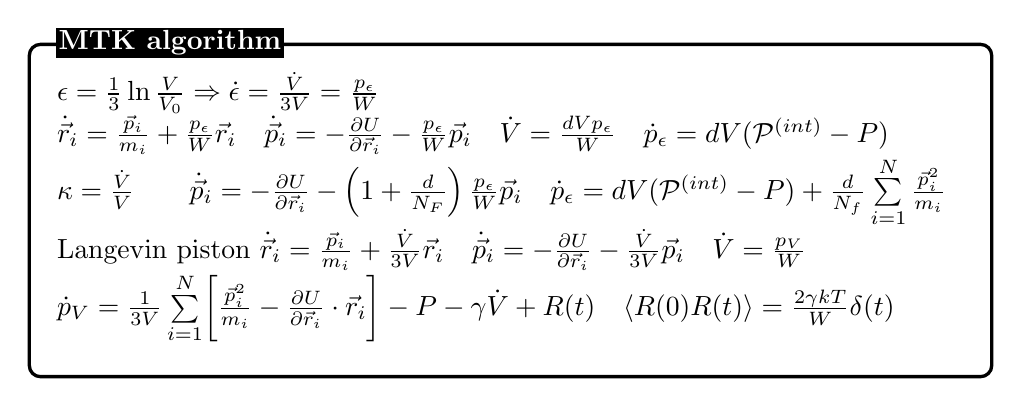
\begin{tikzpicture}
                \node [mybox] (box1){%
                    \begin{minipage}{0.95\textwidth}
                        $\epsilon = \frac{1}{3}\ln\frac{V}{V_0}\Rightarrow\dot{\epsilon} = \frac{\dot{V}}{3V}=\frac{p_\epsilon}{W}$\\
                        $\dot{\vec{r}}_i = \frac{\vec{p}_i}{m_i} + \frac{p_\epsilon}{W}\vec{r}_i\quad\dot{\vec{p}}_i = -\frac{\partial U}{\partial\vec{r}_i} - \frac{p_\epsilon}{W}\vec{p}_i\quad\dot{V} = \frac{dVp_\epsilon}{W}\quad\dot{p}_\epsilon = dV(\mathcal{P}^{(int)}-P)$\\
                        $\kappa = \frac{\dot{V}}{V}\qquad \dot{\vec{p}}_i = -\frac{\partial U}{\partial\vec{r}_i}-\left(1+\frac{d}{N_F}\right)\frac{p_\epsilon}{W}\vec{p}_i\quad\dot{p}_\epsilon = dV(\mathcal{P}^{(int)}-P) + \frac{d}{N_f}\sum\limits_{i=1}^N\frac{\vec{p}_i^2}{m_i}$\\
                        Langevin piston $\dot{\vec{r}}_i = \frac{\vec{p}_i}{m_i} + \frac{\dot{V}}{3V}\vec{r}_i\quad\dot{\vec{p}}_i = -\frac{\partial U}{\partial\vec{r}_i}-\frac{\dot{V}}{3V}\vec{p}_i\quad\dot{V} = \frac{p_V}{W}$\\
                        $\dot{p}_V = \frac{1}{3V}\sum\limits_{i=1}^N\biggl[\frac{\vec{p}_i^2}{m_i}-\frac{\partial U}{\partial\vec{r}_i}\cdot\vec{r}_i\biggr]-P-\gamma\dot{V}+R(t)\quad\langle R(0)R(t)\rangle = \frac{2\gamma kT}{W}\delta(t)$\\
                    \end{minipage}
                };
                \node[fancytitle, inner sep = 1pt, right=10pt] at (box1.north west) {MTK algorithm};
            \end{tikzpicture}
        \end{minipage}
    };
    \node[fancytitle, right=10pt] at (box.north west) {Isobaric ensemble};
\end{tikzpicture}
\begin{tikzpicture}
    \node [mybox] (box){%
        \begin{minipage}{0.233\textwidth}
            \begin{tikzpicture}
                \node [mybox] (box1){%
                    \begin{minipage}{0.95\textwidth}
                        $U(\lambda N, \lambda V, \lambda S) = \lambda U(N, V, S)\Rightarrow U(N, V, S) = \mu N-PV +TS$\\
                        $A(\lambda N, \lambda V, T) = \lambda A(N, V, T)\Rightarrow A(N, V, T) = \mu N-PV$\\
                        $H(\lambda N, \lambda S, P) = \lambda H(N, S, P)\Rightarrow H(N, S, P) = \mu N + TS$\\
                        $G(\lambda N, P, T) = \lambda G(N, P, T)\Rightarrow G(N, P, T) = \mu N$\\
                    \end{minipage}
                };
                \node[fancytitle, inner sep = 1pt, right=10pt] at (box1.north west) {Euler's theorem};
            \end{tikzpicture}
            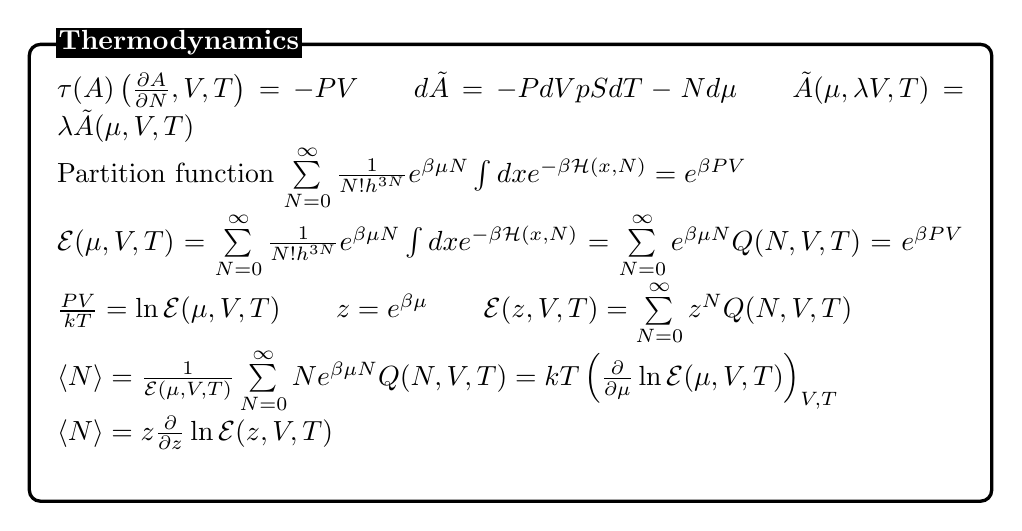
\begin{tikzpicture}
                \node [mybox] (box1){%
                    \begin{minipage}{0.95\textwidth}
                        $\tau(A)\left(\frac{\partial A}{\partial N}, V, T\right) = -PV\qquad d\tilde{A} = -PdVpSdT-Nd\mu\qquad \tilde{A}(\mu, \lambda V, T) = \lambda\tilde{A}(\mu, V, T) $\\
                        Partition function $\sum\limits_{N=0}^{\infty}\frac{1}{N!h^{3N}}e^{\beta\mu N}\int dxe^{-\beta\mathcal{H}(x, N)} = e^{\beta PV}$\\
                        $\mathcal{E}(\mu, V, T) = \sum\limits_{N=0}^{\infty}\frac{1}{N!h^{3N}}e^{\beta\mu N}\int dxe^{-\beta\mathcal{H}(x, N)} = \sum\limits_{N=0}^\infty e^{\beta\mu N}Q(N, V, T) = e^{\beta PV}$
                        $\frac{PV}{kT} = \ln\mathcal{E}(\mu, V, T)\qquad z = e^{\beta\mu}\qquad \mathcal{E}(z, V, T) = \sum\limits_{N=0}^{\infty}z^NQ(N, V, T)$\\
                        $\langle N\rangle = \frac{1}{\mathcal{E}(\mu, V, T)}\sum\limits_{N=0}^{\infty}Ne^{\beta\mu N}Q(N, V, T) = kT\left(\frac{\partial}{\partial\mu}\ln\mathcal{E}(\mu, V, T)\right)_{V, T}$\\
                        $\langle N\rangle = z\frac{\partial}{\partial z}\ln\mathcal{E}(z, V, T)$\\
                    \end{minipage}
                };
                \node[fancytitle, inner sep = 1pt, right=10pt] at (box1.north west) {Thermodynamics};
            \end{tikzpicture}
            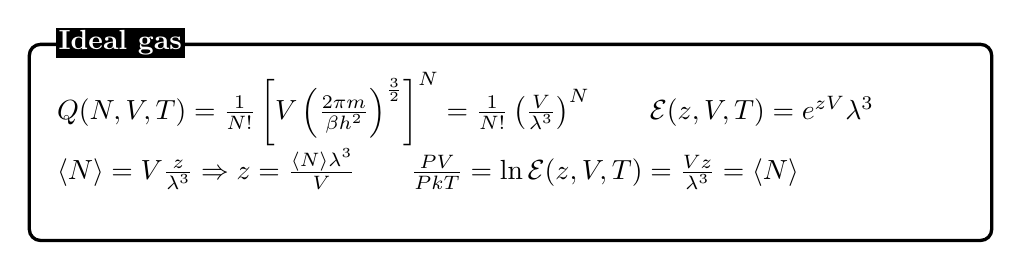
\begin{tikzpicture}
                \node [mybox] (box1){%
                    \begin{minipage}{0.95\textwidth}
                        $Q(N, V, T) = \frac{1}{N!}\left[V\left(\frac{2\pi m}{\beta h^2}\right)^{\frac{3}{2}}\right]^N = \frac{1}{N!}\left(\frac{V}{\lambda^3}\right)^N\qquad\mathcal{E}(z, V, T) = e^{zV}{\lambda^3}$\\
                        $\langle N\rangle = V\frac{z}{\lambda^3}\Rightarrow z = \frac{\langle N\rangle\lambda^3}{V}\qquad\frac{PV}{PkT} = \ln\mathcal{E}(z, V, T) = \frac{Vz}{\lambda^3}=\langle N\rangle$\\
                    \end{minipage}
                };
                \node[fancytitle, inner sep = 1pt, right=10pt] at (box1.north west) {Ideal gas};
            \end{tikzpicture}
            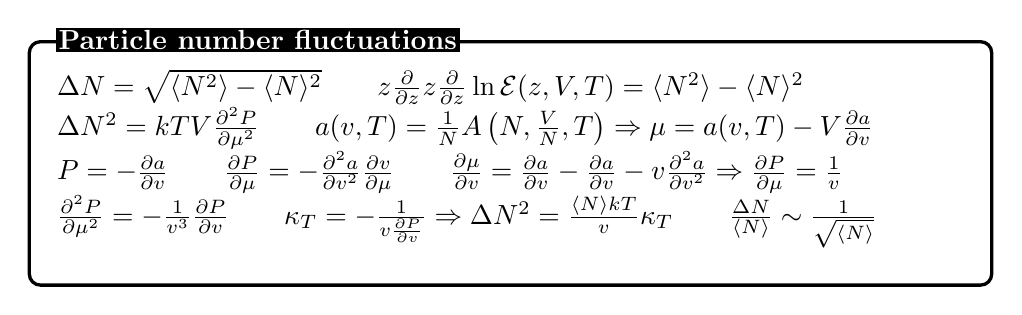
\begin{tikzpicture}
                \node [mybox] (box1){%
                    \begin{minipage}{0.95\textwidth}
                        $\Delta N = \sqrt{\langle N^2\rangle-\langle N\rangle^2}\qquad z\frac{\partial}{\partial z}z\frac{\partial}{\partial z}\ln\mathcal{E}(z, V, T) = \langle N^2\rangle-\langle N\rangle^2$\\
                        $\Delta N^2 = kTV\frac{\partial^2 P}{\partial\mu^2}\qquad a(v, T) = \frac{1}{N}A\left(N, \frac{V}{N}, T\right)\Rightarrow \mu = a(v, T)-V\frac{\partial a}{\partial v}$\\
                        $P = -\frac{\partial a}{\partial v}\qquad\frac{\partial P}{\partial \mu} = -\frac{\partial^2 a}{\partial v^2}\frac{\partial v}{\partial \mu}\qquad \frac{\partial\mu}{\partial v} = \frac{\partial a}{\partial v}-\frac{\partial a}{\partial v}-v\frac{\partial^2a}{\partial v^2}\Rightarrow\frac{\partial P}{\partial \mu} = \frac{1}{v}$\\
                        $\frac{\partial^2 P}{\partial \mu^2} = -\frac{1}{v^3}\frac{\partial P}{\partial{v}}\qquad \kappa_T = -\frac{1}{v\frac{\partial P}{\partial v}}\Rightarrow\Delta N^2 = \frac{\langle N\rangle kT}{v}\kappa_T\qquad \frac{\Delta N}{\langle N\rangle} \sim \frac{1}{\sqrt{\langle N\rangle}}$\\
                    \end{minipage}
                };
                \node[fancytitle, inner sep = 1pt, right=10pt] at (box1.north west) {Particle number fluctuations};
            \end{tikzpicture}
        \end{minipage}
    };
    \node[fancytitle, inner sep = 1pt, right=10pt] at (box.north west) {Grand canonical ensemble};
\end{tikzpicture}
\begin{tikzpicture}
    \node [mybox] (box){%
        \begin{minipage}{0.233\textwidth}
            \begin{tikzpicture}
                \node [mybox] (box1){%
                    \begin{minipage}{0.95\textwidth}
                        $C_f(t') = \frac{\langle(f(x)-\langle f\rangle)(f(t+t')-\langle f\rangle)\rangle}{\sigma^2_f}$\\
                        $C_f(t') = \frac{1}{\sigma^2_f}\frac{1}{N}\sum\limits_{i=1}^{N-\frac{t'}{\Delta t}}(f(j\Delta t)-\langle f\rangle)(f(j\Delta t+t')-\langle f\rangle)\qquad\tau_f = \int_0^{+\infty}dt'C_f(t')$\\
                        $N_f^{ind} \simeq \frac{t_{sim}}{\tau_f}\qquad SE(f) = \frac{\sigma_f}{\sqrt{N_f^{ind}}}\sim\sigma_f\sqrt{\frac{\tau_f}{t_{sim}}}$\\
                    \end{minipage}
                };
                \node[fancytitle, inner sep = 1pt, right=10pt] at (box1.north west) {Autocorrelation analysis};
            \end{tikzpicture}
            \begin{tikzpicture}
                \node [mybox] (box1){%
                    \begin{minipage}{0.95\textwidth}
                        $BSE(f,n) = \frac{\sigma_n}{\sqrt{M}}$\\
                    \end{minipage}
                };
                \node[fancytitle, inner sep = 1pt, right=10pt] at (box1.north west) {Block averaging analysis};
            \end{tikzpicture}
        \end{minipage}
    };
    \node[fancytitle, inner sep = 1pt, right=10pt] at (box.north west) {Quantifying uncertainties and sampling quality};
\end{tikzpicture}
\begin{tikzpicture}
    \node [mybox] (box){%
        \begin{minipage}{0.233\textwidth}
            \begin{tikzpicture}
                \node [mybox] (box1){%
                    \begin{minipage}{0.95\textwidth}
                        $U_{ij} = \gamma_{ij}(\Delta\vec{r}_j-\Delta\vec{r}_j)\cdot(\Delta\vec{r}_j-\Delta\vec{r}_j)=\gamma_{ij}\Delta\vec{r}_{ij}^2\qquad U_{GNM} = \frac{\gamma}{2}\sum\limits_i\sum\limits_j\Delta\vec{r}_{ij}^2$\\
                        $U_{GNM} = \frac{\gamma}{2}\Delta\vec{r}(t)^T\Gamma\Delta\vec{r}(t)\qquad\langle\Delta\vec{r}_i\cdot\Delta\vec{r}_j\rangle=\frac{3kT}{\gamma}\left[\Gamma^{-1}\right]_{ij}$\\
                        $\langle\Delta\vec{r}_i\cdot\Delta\vec{r}_i\rangle = \sum\limits_k[\Delta r_i^2]_k\qquad B_i = \frac{8\pi^2}{3}\langle\Delta r_i^2\rangle$\\
                        Normal mode analysis: $U = \frac{1}{2}\sum\limits_i\sum\limits_jH_{ij}(q_i-q_i^0)(q_j-q_j^0)$\\
                        $\qquad C = \langle\Delta\vec{q}\Delta\vec{q}^T\rangle = \frac{1}{Q}\int\Delta\vec{q}\Delta\vec{q}^Te^{-\frac{\Delta\vec{q}^TH\Delta\vec{q}}{2kT}}d^N\Delta\vec{q} = kTH^{-1}$\\
                    \end{minipage}
                };
                \node[fancytitle, inner sep = 1pt, right=10pt] at (box1.north west) {Gaussian network models};
            \end{tikzpicture}
            \begin{tikzpicture}
                \node [mybox] (box1){%
                    \begin{minipage}{0.95\textwidth}
                        $U_{ANM} = \frac{1}{2}\sum\limits_{ij}\gamma(r_{ij}-r_{ij}^0)^2\Rightarrow\frac{\partial^2U}{\partial x_i\partial x_j} = -\gamma\frac{(x_i-x_j)(y_i-y_j)}{t^2_{ij}}\qquad\langle\Delta\vec{r}_i\cdot\Delta\vec{r}_j\rangle = \frac{3kT}{\gamma}\sum\limits_k\lambda_k^{-1}[\vec{u}_k\vec{u}_k^T]_{ij}$\\
                        Correlation cosine $I_k = \frac{\Delta \vec{q}_{AB}\cdot\vec{u}_k}{|\Delta\vec{q}_{AB}|}\qquad C_0 = \sqrt{\sum\limits_kI_k^2}$\\
                        Degree of connectivity $\kappa_k = N^{-1}e^{-\sum\limits_{i=1}^N\left.\alpha(\Delta r_i)^2\right\vert_k\left.\log(\alpha(\Delta r_i)^2\right\vert_k)}\qquad \sum\limits_{i=1}^N\left.\alpha(\Delta r_i)^2\right\vert_k=1$\\
                    \end{minipage}
                };
                \node[fancytitle, inner sep = 1pt, right=10pt] at (box1.north west) {Anisotropic network model};
            \end{tikzpicture}
            \begin{tikzpicture}
                \node [mybox] (box1){%
                    \begin{minipage}{0.95\textwidth}
                        Covariance matrix $C_{ij} = \overline{(x_i(t)-\overline{x_i(t)})(x_j(t)-\overline{x_j(t)})}$\\
                        Correlation matrix $R_{ij} = \frac{\overline{(x_i(t)-\overline{x_i(t)})(x_j(t)-\overline{x_j(t)})}}{\sigma_{x_i}\sigma_{x_j}}$\\
                        $PC_k(t) = \sum\limits_{i=1}^N\vec{d}_i(t)\cdot\vec{u}_i^k\quad c_k = \frac{2}{T_{sim}}\left(\int_0^{T_{sim}}\cos\left(\pi\frac{k_BT}{\lambda_k}t\right)PC_k(t)dt\right)^2\left(\int_0^{T_{sim}}PC_k^2(t)dt\right)^{-1}$\\
                        $\Omega_{A, B} = 1-\left[\frac{\sum\limits_{k=1}^{3N-6}(\lambda_k^A+\lambda_k^B)-2\sum\limits_{k=1}^{3N-6}\sum\limits_{j=1}^{3N-6}\sqrt{\lambda_k^A\lambda_j^B}(\vec{u}_k^A\cdot\vec{u}_j^B)^2}{\sum\limits_{k=1}^{3N-6}(\lambda_k^A+\lambda_k^B)}\right]^{\frac{1}{2}}$\\

                    \end{minipage}
                };
                \node[fancytitle, inner sep = 1pt, right=10pt] at (box1.north west) {Essential dynamics};
            \end{tikzpicture}
        \end{minipage}
    };
    \node[fancytitle, inner sep = 1pt, right=10pt] at (box.north west) {Protein motions};
\end{tikzpicture}
\begin{tikzpicture}
    \node [mybox] (box){%
        \begin{minipage}{0.233\textwidth}
            \begin{tikzpicture}
                \node [mybox] (box1){%
                    \begin{minipage}{0.95\textwidth}
                        $f(x) \ge 0\land\int f(x)dx = 1\qquad I = \int dx\phi(x)f(x)\equiv\langle\phi\rangle_f$\\
                        $\tilde{I}_M = \frac{1}{M}\int_{i=1}^M\phi(x_i)\qquad\lim\limits_{M\to\infty}\tilde{I}_M = I$\\
                        $\int dx\phi(x)f(x) = \frac{1}{M}\int_{i=1}^M\phi(x_i)\pm\frac{1}{\sqrt{M}}\left[\langle\phi^2\rangle_f-\langle\phi\rangle_f^2\right]^{\frac{1}{2}}$\\
                        $P(X) = \int_a^Xf(x)dx\quad f(X) = \frac{dP}{dX}\quad X\ge x\Rightarrow g(X)\ge g(x)\quad \tilde{P}(Y=g(X)) = P(X)$\\
                    \end{minipage}
                };
                \node[fancytitle, inner sep = 1pt, right=10pt] at (box1.north west) {Introduction};
            \end{tikzpicture}
        \end{minipage}
    };
    \node[fancytitle, inner sep = 1pt, right=10pt] at (box.north west) {Monte Carlo methods};
\end{tikzpicture}
\begin{tikzpicture}
    \node [mybox] (box){%
        \begin{minipage}{0.233\textwidth}
            \begin{tikzpicture}
                \node [mybox] (box1){%
                    \begin{minipage}{0.95\textwidth}
                        $I = \int dx\phi(x)f(x) = \int dx\left[\frac{\phi(x)f(x)}{h(x)}\right]h(x) = \int dx\psi(x)h(x) = \frac{1}{M}\sum\limits_{i=1}^M\psi(x_i)\pm\frac{1}{\sqrt{M}}\left[\langle\psi^2\rangle_h-\langle\psi\rangle_h^2\right]^{\frac{1}{2}}$\\
                        $\sigma^2[h] = \int dx\frac{\phi^2(x)f^2(x)}{h(x)}-\left[\int dx\phi(x)f(x)\right]^2$\\
                        $\delta F[h] = -\frac{\phi^2(x)f^2(x)}{h^2(x)}\delta h(x)-\lambda\delta h(x)\qquad \frac{\delta F[h]}{\delta h(x)} = 0\Rightarrow h(x) = \frac{1}{\sqrt{-\lambda}}\phi(x)f(x)$\\
                    \end{minipage}
                };
                \node[fancytitle, inner sep = 1pt, right=10pt] at (box1.north west) {Importance sampling};
            \end{tikzpicture}
            \begin{tikzpicture}
                \node [mybox] (box1){%
                    \begin{minipage}{0.95\textwidth}
                        Detailed balance $R(x|y)f(y) = R(y|x)f(x)$\\
                        Rejection method $R(x|y) = A(x|y)T(x|y)\qquad r(x|y) = \frac{T(y|x)f(x)}{T(x|y)f(y)}$\\
                        $\qquad A(x|y) = \min[1, r(x|y)]$\\
                        Metropolis algorithm $r(x_{k+1}|x_k) = \frac{T(x_k|x_{k+1})f(x_{k+1})}{T(x_{k+1}|x_k)f(x_k)}$\\
                        Canonical distribution $A(r'|r) = \min\left[1,e^{-\beta(U(r')-U(r))}\right]$\\
                        Trial move $\begin{cases} x'_i = x_i+\frac{1}{\sqrt{3}}(\xi_x-0.5)\Delta\\y'_i = y_i+\frac{1}{\sqrt{3}}(\xi_y-0.5)\Delta\\z'_i = z_i+\frac{1}{\sqrt{3}}(\xi_z-0.5)\Delta\end{cases}$\\
                        Isothermal-isobaric $A(V'|V) = \min\left[1, e^{-\beta P(V'-V)}e^{N\ln\frac{V'}{V}}e^{-\beta(U(r')-I)}\right]$\\
                        Gran canonical $\begin{cases} A(N+1|N) = min\left[1, \frac{V}{\lambda^3(N+1)}e^{\beta\mu}e^{-\beta(U(r')-U(r))}\right]\\A(N-1|N) = \min\left[1,\frac{\lambda^3 N}{V}e^{-\beta\mu}e^{-\beta(U(r')-U(r))}\right]\end{cases}$\\
                    \end{minipage}
                };
                \node[fancytitle, inner sep = 1pt, right=10pt] at (box1.north west) {Markov chains};
            \end{tikzpicture}
            \begin{tikzpicture}
                \node [mybox] (box1){%
                    \begin{minipage}{0.95\textwidth}
                        $A(r', p'|r, p) = \min\left[1, e^{-\beta\Delta\mathcal{H}}\right]\qquad T(r', p'|r, p) = T(r,-p|r', -p')$\\
                        $\int d^Npd^Np' T(r',p'|r,p)A(r', p'|r,p)f(r,p) = \int d^Npd^Np' T(r, p|r', p')A(r,p|r',p')f(r',p')$\\
                    \end{minipage}
                };
                \node[fancytitle, inner sep = 1pt, right=10pt] at (box1.north west) {Hybrid Monte Carlo};
            \end{tikzpicture}
        \end{minipage}
    };
    \node[fancytitle, inner sep = 1pt, right=10pt] at (box.north west) {Monte Carlo methods (contd)};
\end{tikzpicture}
\begin{tikzpicture}
    \node [mybox] (box){%
        \begin{minipage}{0.233\textwidth}
            \begin{tikzpicture}
                \node [mybox] (box1){%
                    \begin{minipage}{0.95\textwidth}
                        $\Delta A_{AB} = -kT\ln\frac{Z_B}{Z_A}\qquad \frac{Z_B}{Z_A} = \left\langle e^{-\beta[U_B(\vec{r}_1, \dots, \vec{r}_N)-U_A(\vec{r}_1, \dots, \vec{r}_N)]}\right\rangle_A$\\
                        $\Delta A_{AB} = -kT\ln\left\langle e^{-\beta[U_B(\vec{r}_1, \dots, \vec{r}_N)-U_A(\vec{r}_1, \dots, \vec{r}_N)]}\right\rangle_A$\\
                        Adiabatic switching: $\frac{kT}{Z}\frac{\partial Z}{\partial\lambda} = \frac{kT}{Z}\int d^N\vec{r}\left(-\beta\frac{\partial U}{\partial\lambda}\right)e^{-\beta U(\vec{r}_1, \dots, \vec{r}_N)} = -\langle\frac{\partial U}{\partial\lambda}\rangle$\\
                        Thermodynamics integration: $\Delta A_{AB} = \int_0^1\left(\frac{\partial A}{\partial \lambda}\right)d\lambda = \int_0^1\left\langle\frac{\partial U}{\partial\lambda}\right\rangle_\lambda d\lambda$\\
                        Adiabatic free energy dynamics: $\left\langle\frac{p_\lambda^2}{2m_\lambda}\right\rangle = kT_\lambda\qquad Z(\lambda, \beta) = \int d^N\vec{r}e^{-\beta U(\vec{r}, \lambda)}$\\
                        $\mathcal{H}_{eff}(\lambda, p_\lambda) = \frac{p_\lambda^2}{2m_\lambda}-\frac{1}{\beta}\ln Z(\lambda, \beta)\qquad \tilde{P}_{adb}(\lambda, \beta, \beta_\lambda) = \left[Z(\lambda, \beta)\right]^{\frac{\beta_\lambda}{\beta}}$\\
                        $A(\lambda) = -kT\ln Z(\lambda, \beta) + const$\\
                    \end{minipage}
                };
                \node[fancytitle, inner sep = 1pt, right=10pt] at (box1.north west) {Free energy perturbation theory};
            \end{tikzpicture}
            \begin{tikzpicture}
                \node [mybox] (box1){%
                    \begin{minipage}{0.95\textwidth}
                        $W_{AB} = \langle\mathcal{W}_{AB}(x)\rangle_A \ge \Delta A_{AB}\qquad \langle e^{-\beta\mathcal{W}_{AB}(x_0)}\rangle_A = e^{-\beta\Delta A_{AB}}$\\
                        Pulling experiment: $U(\vec{r}_1, \dots, \vec{r}_N, t) = U_0(\vec{r}_1, \dots, \vec{r}_N) + \frac{1}{2}k(|\vec{r}_1-\vec{r}_N|-r_{eq}-vt)^2$\\
                        $\langle e^{-\beta\mathcal{W}_\tau}\rangle = \int\mathcal{W}_\tau P(\mathcal{W}_\tau)e^{-\beta\mathcal{W}_\tau}$\\
                        $P(\mathcal{W}_\tau)\sim N\Rightarrow \ln\langle e^{-\beta\mathcal{W}_\tau}\simeq -\beta\langle\mathcal{W}_\tau\rangle + \frac{\beta^2}{2}(\langle\mathcal{W}_\tau^2\rangle - \langle\mathcal{W}_\tau\rangle^2)$\\
                    \end{minipage}
                };
                \node[fancytitle, inner sep = 1pt, right=10pt] at (box1.north west) {Jarzynski's equality};
            \end{tikzpicture}
            \begin{tikzpicture}
                \node [mybox] (box1){%
                    \begin{minipage}{0.95\textwidth}
                        $F\left(\vec{r}^{(1)}, \dots, \vec{r}^{(M)}\right) = \prod\limits_{K=1}^Mf_K\left(\vec{r}^{(K)}\right)\qquad f_K\left(\vec{r}^{(K)}\right) = \frac{e^{-\beta_K U\left(\vec{r}^{(K)}\right)}}{Q(N, V, T_K}$\\
                        $T\left(\tilde{\vec{r}}^{(K)}, \tilde{\vec{r}}^{(K+1)}|\vec{r}^{(K)}, \vec{r}^{(K+1)}\right) = T\left(\vec{r}^{(K)}, \vec{r}^{(K+1)}|\tilde{\vec{r}}^{(K)}, \tilde{\vec{r}}^{(K+1)}\right)$\\
                        $A(\vec{r}^{(K+1)}, \vec{r}^{(K)} | \vec{r}^{(K)}, \vec{r}^{(K+1)}) = \min\left[1, e^{-\Delta_{K, K+1}}\right]$\\
                        $\Delta_{K, K+1} = (\beta_K-\beta_{K +1})\left[U\left(\vec{r}^{(K+1)}\right)-U\left(\vec{r}^{(K)}\right)\right]$\\
                        Wang-Landau sampling $Q(\beta) = \int_0^{\infty}dE e^{-\beta E}\Omega(E)\qquad A(E_2|E_1) = \min\left[1, \frac{\Omega(E_2)}{\Omega(E_1)}\right]$\\
                    \end{minipage}
                };
                \node[fancytitle, inner sep = 1pt, right=10pt] at (box1.north west) {Replica exchange Monte Carlo};
            \end{tikzpicture}
        \end{minipage}
    };
    \node[fancytitle, inner sep = 1pt, right=10pt] at (box.north west) {Free energy calculations};
\end{tikzpicture}
\end{multicols*}
\end{document}
